\documentclass[twoside]{book}

% Packages required by doxygen
\usepackage{fixltx2e}
\usepackage{calc}
\usepackage{doxygen}
\usepackage{graphicx}
\usepackage[utf8]{inputenc}
\usepackage{makeidx}
\usepackage{multicol}
\usepackage{multirow}
\PassOptionsToPackage{warn}{textcomp}
\usepackage{textcomp}
\usepackage[nointegrals]{wasysym}
\usepackage[table]{xcolor}

% Font selection
\usepackage[T1]{fontenc}
\usepackage{mathptmx}
\usepackage[scaled=.90]{helvet}
\usepackage{courier}
\usepackage{amssymb}
\usepackage{sectsty}
\renewcommand{\familydefault}{\sfdefault}
\allsectionsfont{%
  \fontseries{bc}\selectfont%
  \color{darkgray}%
}
\renewcommand{\DoxyLabelFont}{%
  \fontseries{bc}\selectfont%
  \color{darkgray}%
}
\newcommand{\+}{\discretionary{\mbox{\scriptsize$\hookleftarrow$}}{}{}}

% Page & text layout
\usepackage{geometry}
\geometry{%
  letterpaper,%
  top=2.5cm,%
  bottom=2.5cm,%
  left=2.5cm,%
  right=2.5cm%
}
\tolerance=750
\hfuzz=15pt
\hbadness=750
\setlength{\emergencystretch}{15pt}
\setlength{\parindent}{0cm}
\setlength{\parskip}{0.2cm}
\makeatletter
\renewcommand{\paragraph}{%
  \@startsection{paragraph}{4}{0ex}{-1.0ex}{1.0ex}{%
    \normalfont\normalsize\bfseries\SS@parafont%
  }%
}
\renewcommand{\subparagraph}{%
  \@startsection{subparagraph}{5}{0ex}{-1.0ex}{1.0ex}{%
    \normalfont\normalsize\bfseries\SS@subparafont%
  }%
}
\makeatother

% Headers & footers
\usepackage{fancyhdr}
\pagestyle{fancyplain}
\fancyhead[LE]{\fancyplain{}{\bfseries\thepage}}
\fancyhead[CE]{\fancyplain{}{}}
\fancyhead[RE]{\fancyplain{}{\bfseries\leftmark}}
\fancyhead[LO]{\fancyplain{}{\bfseries\rightmark}}
\fancyhead[CO]{\fancyplain{}{}}
\fancyhead[RO]{\fancyplain{}{\bfseries\thepage}}
\fancyfoot[LE]{\fancyplain{}{}}
\fancyfoot[CE]{\fancyplain{}{}}
\fancyfoot[RE]{\fancyplain{}{\bfseries\scriptsize Generated on Wed May 4 2016 14\+:19\+:06 for Option Pricing Example by Doxygen }}
\fancyfoot[LO]{\fancyplain{}{\bfseries\scriptsize Generated on Wed May 4 2016 14\+:19\+:06 for Option Pricing Example by Doxygen }}
\fancyfoot[CO]{\fancyplain{}{}}
\fancyfoot[RO]{\fancyplain{}{}}
\renewcommand{\footrulewidth}{0.4pt}
\renewcommand{\chaptermark}[1]{%
  \markboth{#1}{}%
}
\renewcommand{\sectionmark}[1]{%
  \markright{\thesection\ #1}%
}

% Indices & bibliography
\usepackage{natbib}
\usepackage[titles]{tocloft}
\setcounter{tocdepth}{3}
\setcounter{secnumdepth}{5}
\makeindex

% Packages requested by user
\usepackage{amsfonts}

% Hyperlinks (required, but should be loaded last)
\usepackage{ifpdf}
\ifpdf
  \usepackage[pdftex,pagebackref=true]{hyperref}
\else
  \usepackage[ps2pdf,pagebackref=true]{hyperref}
\fi
\hypersetup{%
  colorlinks=true,%
  linkcolor=blue,%
  citecolor=blue,%
  unicode%
}

% Custom commands
\newcommand{\clearemptydoublepage}{%
  \newpage{\pagestyle{empty}\cleardoublepage}%
}


%===== C O N T E N T S =====

\begin{document}

% Titlepage & ToC
\hypersetup{pageanchor=false,
             bookmarks=true,
             bookmarksnumbered=true,
             pdfencoding=unicode
            }
\pagenumbering{roman}
\begin{titlepage}
\vspace*{7cm}
\begin{center}%
{\Large Option Pricing Example }\\
\vspace*{1cm}
{\large Generated by Doxygen 1.8.8}\\
\vspace*{0.5cm}
{\small Wed May 4 2016 14:19:06}\\
\end{center}
\end{titlepage}
\clearemptydoublepage
\tableofcontents
\clearemptydoublepage
\pagenumbering{arabic}
\hypersetup{pageanchor=true}

%--- Begin generated contents ---
\chapter{Introduction}
\label{index}\hypertarget{index}{}A typical reason for studying parabolic partial differential equations in finance is the Black--Scholes equation.

Let $ S(t) $ denote the price at time $ t $ of the underlying asset under the Black--Scholes equation. Suppose that at time $ t $ the price of a financial derivative $ H(t) $ can be expressed using a function $ u $, defined as\+: \[ H(t) = u(t, S (t)). \] If $ u $ is a $ C^{1,2} $ function on $ [0,T)\times \mathbb{R} $, then the Black--Scholes equation can be used to solve for $ u $.

In this project, we study how to construct a minimal framework to encode the mechanisms implementing a standard finite difference explicit method to solve the time-\/dependent portion of the Black--Scholes equation. For the ''spatial'' component, we also use standard finite differences. We use a second-\/order of numerical accuracy, and we use a nodal grid.

Future work includes comparing these results with actual data and also compare these results with an approach based on mimetic finite differences.

\begin{DoxySeeAlso}{See also}
This code is also listed and fully explained in the book Numerical Methods in Finance with C++ by Maciej Capiński and Tomasz Zastawniak, published in September 2012.
\end{DoxySeeAlso}
\begin{DoxyWarning}{Warning}
This code is a minimally-\/complete example intended for research and modeling. This is not intended to be production code. 
\end{DoxyWarning}

\chapter{Read Me File}
\label{page_readme}
\hypertarget{page_readme}{}

\begin{DoxyVerbInclude}
# OptionPricing

This repository contains object-oriented code implementing numerical methods for
option pricing.

This code is also listed and fully explained in the book **Numerical Methods in
Finance with C++** by Maciej Capiński and Tomasz Zastawniak, published in
September 2012.

This code is a minimally-complete example intended for research and modeling.
This is not intended to be production code.
\end{DoxyVerbInclude}
 
\chapter{Tested Architectures}
\label{page_architectures}
\hypertarget{page_architectures}{}
The following architectures have provided a correct execution of this code\+:

\begin{DoxyVerb}1. Intel(R) Core(TM) i7-4600U CPU 2.10 GHz 4096 KB of cache and a stepping of 1.
   Linux 3.16.7-29-desktop #1 SMP PREEMPT (6be6a97) x86_64 GNU/Linux
   openSUSE 13.2 (Harlequin) (x86_64)
   gcc (SUSE Linux) 4.8.3 20140627 [gcc-4_8-branch revision 212064]
\end{DoxyVerb}
 
\chapter{Hierarchical Index}
\section{Class Hierarchy}
This inheritance list is sorted roughly, but not completely, alphabetically\+:\begin{DoxyCompactList}
\item \contentsline{section}{B\+S\+Model}{\pageref{classBSModel}}{}
\item \contentsline{section}{F\+D\+Method}{\pageref{classFDMethod}}{}
\begin{DoxyCompactList}
\item \contentsline{section}{Explicit\+Method}{\pageref{classExplicitMethod}}{}
\end{DoxyCompactList}
\item \contentsline{section}{Option}{\pageref{classOption}}{}
\begin{DoxyCompactList}
\item \contentsline{section}{Put}{\pageref{classPut}}{}
\end{DoxyCompactList}
\item \contentsline{section}{Parab\+P\+D\+E}{\pageref{classParabPDE}}{}
\begin{DoxyCompactList}
\item \contentsline{section}{B\+S\+Eq}{\pageref{classBSEq}}{}
\end{DoxyCompactList}
\end{DoxyCompactList}

\chapter{Class Index}
\section{Class List}
Here are the classes, structs, unions and interfaces with brief descriptions\+:\begin{DoxyCompactList}
\item\contentsline{section}{\hyperlink{classBSEq}{B\+S\+Eq} }{\pageref{classBSEq}}{}
\item\contentsline{section}{\hyperlink{classBSModel}{B\+S\+Model} }{\pageref{classBSModel}}{}
\item\contentsline{section}{\hyperlink{classExplicitMethod}{Explicit\+Method} }{\pageref{classExplicitMethod}}{}
\item\contentsline{section}{\hyperlink{classFDMethod}{F\+D\+Method} }{\pageref{classFDMethod}}{}
\item\contentsline{section}{\hyperlink{classOption}{Option} }{\pageref{classOption}}{}
\item\contentsline{section}{\hyperlink{classParabPDE}{Parab\+P\+D\+E} }{\pageref{classParabPDE}}{}
\item\contentsline{section}{\hyperlink{classPut}{Put} }{\pageref{classPut}}{}
\end{DoxyCompactList}

\chapter{File Index}
\section{File List}
Here is a list of all files with brief descriptions\+:\begin{DoxyCompactList}
\item\contentsline{section}{\hyperlink{BSEq_8cpp}{B\+S\+Eq.\+cpp} \\*Implements a class representing the Black--Scholes equation }{\pageref{BSEq_8cpp}}{}
\item\contentsline{section}{\hyperlink{BSEq_8h}{B\+S\+Eq.\+h} \\*Defines a class representing the Black--Scholes equation }{\pageref{BSEq_8h}}{}
\item\contentsline{section}{\hyperlink{BSModel01_8cpp}{B\+S\+Model01.\+cpp} \\*Implementation of a class using the Box--Muller method for sample paths }{\pageref{BSModel01_8cpp}}{}
\item\contentsline{section}{\hyperlink{BSModel01_8h}{B\+S\+Model01.\+h} \\*Definition of a class using the Box--Muller method for sample paths }{\pageref{BSModel01_8h}}{}
\item\contentsline{section}{\hyperlink{ExplicitMethod_8cpp}{Explicit\+Method.\+cpp} }{\pageref{ExplicitMethod_8cpp}}{}
\item\contentsline{section}{\hyperlink{ExplicitMethod_8h}{Explicit\+Method.\+h} }{\pageref{ExplicitMethod_8h}}{}
\item\contentsline{section}{\hyperlink{FDMethod_8cpp}{F\+D\+Method.\+cpp} }{\pageref{FDMethod_8cpp}}{}
\item\contentsline{section}{\hyperlink{FDMethod_8h}{F\+D\+Method.\+h} }{\pageref{FDMethod_8h}}{}
\item\contentsline{section}{\hyperlink{Main24_8cpp}{Main24.\+cpp} \\*Test the option pricing code based on the Black--Scholes model }{\pageref{Main24_8cpp}}{}
\item\contentsline{section}{\hyperlink{Options_8cpp}{Options.\+cpp} \\*Implementation of classes to represent an option an a put option }{\pageref{Options_8cpp}}{}
\item\contentsline{section}{\hyperlink{Options_8h}{Options.\+h} \\*Definition of classes to represent an option an a put option }{\pageref{Options_8h}}{}
\item\contentsline{section}{\hyperlink{ParabPDE_8h}{Parab\+P\+D\+E.\+h} \\*Definition of a class for parabolic partial differential equations }{\pageref{ParabPDE_8h}}{}
\end{DoxyCompactList}

\chapter{Class Documentation}
\hypertarget{classBSEq}{\section{B\+S\+Eq Class Reference}
\label{classBSEq}\index{B\+S\+Eq@{B\+S\+Eq}}
}


{\ttfamily \#include $<$B\+S\+Eq.\+h$>$}



Inheritance diagram for B\+S\+Eq\+:\nopagebreak
\begin{figure}[H]
\begin{center}
\leavevmode
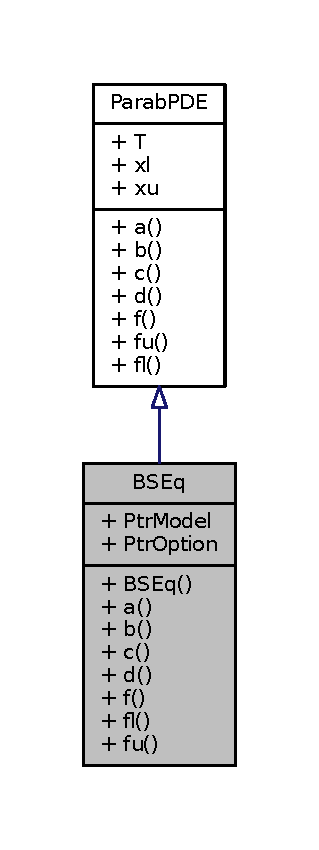
\includegraphics[width=153pt]{classBSEq__inherit__graph}
\end{center}
\end{figure}


Collaboration diagram for B\+S\+Eq\+:\nopagebreak
\begin{figure}[H]
\begin{center}
\leavevmode
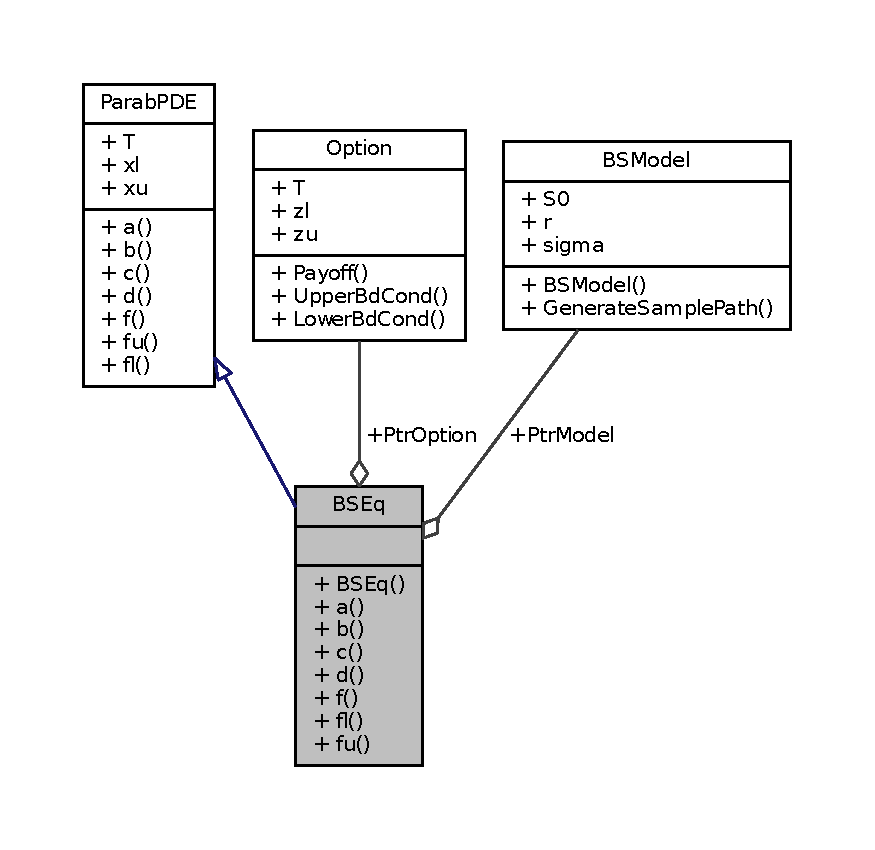
\includegraphics[width=350pt]{classBSEq__coll__graph}
\end{center}
\end{figure}
\subsection*{Public Member Functions}
\begin{DoxyCompactItemize}
\item 
\hyperlink{classBSEq_a3545b5fe078c573514666f07e3d516b2}{B\+S\+Eq} (\hyperlink{classBSModel}{B\+S\+Model} $\ast$Ptr\+Model\+\_\+, \hyperlink{classOption}{Option} $\ast$Ptr\+Option\+\_\+)
\item 
double \hyperlink{classBSEq_aac9b72618a86b764022bc2f8a0623b0c}{a} (double t, double z)
\item 
double \hyperlink{classBSEq_a7b0a00c216ae383f5a768c8efd42e672}{b} (double t, double z)
\item 
double \hyperlink{classBSEq_aa63fc29fedf4ef53ace9499fab4d7aba}{c} (double t, double z)
\item 
double \hyperlink{classBSEq_ae01526739bc51e813dfdb880585aefc0}{d} (double t, double z)
\item 
double \hyperlink{classBSEq_a6c81cef2ec102bc86bc8ff6378a2a519}{f} (double z)
\item 
double \hyperlink{classBSEq_a5bde9ad3db5d94df77c78929de7f2717}{fl} (double t)
\item 
double \hyperlink{classBSEq_acebc22c41d04659861ef346d988de565}{fu} (double t)
\end{DoxyCompactItemize}
\subsection*{Public Attributes}
\begin{DoxyCompactItemize}
\item 
\hyperlink{classBSModel}{B\+S\+Model} $\ast$ \hyperlink{classBSEq_a44b63f8349d8ab91a1fb8fc026cdf142}{Ptr\+Model}
\item 
\hyperlink{classOption}{Option} $\ast$ \hyperlink{classBSEq_a280b15d8a4cd19d1aefc9feeb35a75bb}{Ptr\+Option}
\end{DoxyCompactItemize}


\subsection{Detailed Description}


Definition at line \hyperlink{BSEq_8h_source_l00057}{57} of file \hyperlink{BSEq_8h_source}{B\+S\+Eq.\+h}.



\subsection{Constructor \& Destructor Documentation}
\hypertarget{classBSEq_a3545b5fe078c573514666f07e3d516b2}{\index{B\+S\+Eq@{B\+S\+Eq}!B\+S\+Eq@{B\+S\+Eq}}
\index{B\+S\+Eq@{B\+S\+Eq}!B\+S\+Eq@{B\+S\+Eq}}
\subsubsection[{B\+S\+Eq}]{\setlength{\rightskip}{0pt plus 5cm}B\+S\+Eq\+::\+B\+S\+Eq (
\begin{DoxyParamCaption}
\item[{{\bf B\+S\+Model} $\ast$}]{Ptr\+Model\+\_\+, }
\item[{{\bf Option} $\ast$}]{Ptr\+Option\+\_\+}
\end{DoxyParamCaption}
)}}\label{classBSEq_a3545b5fe078c573514666f07e3d516b2}


Definition at line \hyperlink{BSEq_8cpp_source_l00054}{54} of file \hyperlink{BSEq_8cpp_source}{B\+S\+Eq.\+cpp}.



\subsection{Member Function Documentation}
\hypertarget{classBSEq_aac9b72618a86b764022bc2f8a0623b0c}{\index{B\+S\+Eq@{B\+S\+Eq}!a@{a}}
\index{a@{a}!B\+S\+Eq@{B\+S\+Eq}}
\subsubsection[{a}]{\setlength{\rightskip}{0pt plus 5cm}double B\+S\+Eq\+::a (
\begin{DoxyParamCaption}
\item[{double}]{t, }
\item[{double}]{z}
\end{DoxyParamCaption}
)\hspace{0.3cm}{\ttfamily [virtual]}}}\label{classBSEq_aac9b72618a86b764022bc2f8a0623b0c}


Implements \hyperlink{classParabPDE_a809e251d53ff62714bc8a30e45cc88a5}{Parab\+P\+D\+E}.



Definition at line \hyperlink{BSEq_8cpp_source_l00063}{63} of file \hyperlink{BSEq_8cpp_source}{B\+S\+Eq.\+cpp}.

\hypertarget{classBSEq_a7b0a00c216ae383f5a768c8efd42e672}{\index{B\+S\+Eq@{B\+S\+Eq}!b@{b}}
\index{b@{b}!B\+S\+Eq@{B\+S\+Eq}}
\subsubsection[{b}]{\setlength{\rightskip}{0pt plus 5cm}double B\+S\+Eq\+::b (
\begin{DoxyParamCaption}
\item[{double}]{t, }
\item[{double}]{z}
\end{DoxyParamCaption}
)\hspace{0.3cm}{\ttfamily [virtual]}}}\label{classBSEq_a7b0a00c216ae383f5a768c8efd42e672}


Implements \hyperlink{classParabPDE_ab98c81bf66471fa6f67dc17b9123bda6}{Parab\+P\+D\+E}.



Definition at line \hyperlink{BSEq_8cpp_source_l00068}{68} of file \hyperlink{BSEq_8cpp_source}{B\+S\+Eq.\+cpp}.

\hypertarget{classBSEq_aa63fc29fedf4ef53ace9499fab4d7aba}{\index{B\+S\+Eq@{B\+S\+Eq}!c@{c}}
\index{c@{c}!B\+S\+Eq@{B\+S\+Eq}}
\subsubsection[{c}]{\setlength{\rightskip}{0pt plus 5cm}double B\+S\+Eq\+::c (
\begin{DoxyParamCaption}
\item[{double}]{t, }
\item[{double}]{z}
\end{DoxyParamCaption}
)\hspace{0.3cm}{\ttfamily [virtual]}}}\label{classBSEq_aa63fc29fedf4ef53ace9499fab4d7aba}


Implements \hyperlink{classParabPDE_aebec9339309e456136ecd0c3b4a74bb0}{Parab\+P\+D\+E}.



Definition at line \hyperlink{BSEq_8cpp_source_l00073}{73} of file \hyperlink{BSEq_8cpp_source}{B\+S\+Eq.\+cpp}.

\hypertarget{classBSEq_ae01526739bc51e813dfdb880585aefc0}{\index{B\+S\+Eq@{B\+S\+Eq}!d@{d}}
\index{d@{d}!B\+S\+Eq@{B\+S\+Eq}}
\subsubsection[{d}]{\setlength{\rightskip}{0pt plus 5cm}double B\+S\+Eq\+::d (
\begin{DoxyParamCaption}
\item[{double}]{t, }
\item[{double}]{z}
\end{DoxyParamCaption}
)\hspace{0.3cm}{\ttfamily [virtual]}}}\label{classBSEq_ae01526739bc51e813dfdb880585aefc0}


Implements \hyperlink{classParabPDE_a13531e677a97660f56f88fc8a9f2c593}{Parab\+P\+D\+E}.



Definition at line \hyperlink{BSEq_8cpp_source_l00078}{78} of file \hyperlink{BSEq_8cpp_source}{B\+S\+Eq.\+cpp}.

\hypertarget{classBSEq_a6c81cef2ec102bc86bc8ff6378a2a519}{\index{B\+S\+Eq@{B\+S\+Eq}!f@{f}}
\index{f@{f}!B\+S\+Eq@{B\+S\+Eq}}
\subsubsection[{f}]{\setlength{\rightskip}{0pt plus 5cm}double B\+S\+Eq\+::f (
\begin{DoxyParamCaption}
\item[{double}]{z}
\end{DoxyParamCaption}
)\hspace{0.3cm}{\ttfamily [virtual]}}}\label{classBSEq_a6c81cef2ec102bc86bc8ff6378a2a519}


Implements \hyperlink{classParabPDE_a099b6ba266fb033de9901a60dc935ddf}{Parab\+P\+D\+E}.



Definition at line \hyperlink{BSEq_8cpp_source_l00083}{83} of file \hyperlink{BSEq_8cpp_source}{B\+S\+Eq.\+cpp}.



Here is the call graph for this function\+:\nopagebreak
\begin{figure}[H]
\begin{center}
\leavevmode
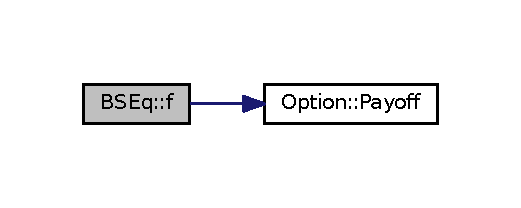
\includegraphics[width=250pt]{classBSEq_a6c81cef2ec102bc86bc8ff6378a2a519_cgraph}
\end{center}
\end{figure}


\hypertarget{classBSEq_a5bde9ad3db5d94df77c78929de7f2717}{\index{B\+S\+Eq@{B\+S\+Eq}!fl@{fl}}
\index{fl@{fl}!B\+S\+Eq@{B\+S\+Eq}}
\subsubsection[{fl}]{\setlength{\rightskip}{0pt plus 5cm}double B\+S\+Eq\+::fl (
\begin{DoxyParamCaption}
\item[{double}]{t}
\end{DoxyParamCaption}
)\hspace{0.3cm}{\ttfamily [virtual]}}}\label{classBSEq_a5bde9ad3db5d94df77c78929de7f2717}


Implements \hyperlink{classParabPDE_aa083d2745f44daba57ad296749eb7ec0}{Parab\+P\+D\+E}.



Definition at line \hyperlink{BSEq_8cpp_source_l00088}{88} of file \hyperlink{BSEq_8cpp_source}{B\+S\+Eq.\+cpp}.



Here is the call graph for this function\+:\nopagebreak
\begin{figure}[H]
\begin{center}
\leavevmode
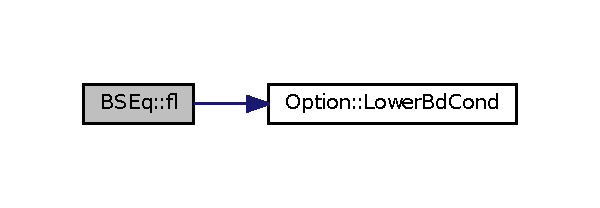
\includegraphics[width=288pt]{classBSEq_a5bde9ad3db5d94df77c78929de7f2717_cgraph}
\end{center}
\end{figure}


\hypertarget{classBSEq_acebc22c41d04659861ef346d988de565}{\index{B\+S\+Eq@{B\+S\+Eq}!fu@{fu}}
\index{fu@{fu}!B\+S\+Eq@{B\+S\+Eq}}
\subsubsection[{fu}]{\setlength{\rightskip}{0pt plus 5cm}double B\+S\+Eq\+::fu (
\begin{DoxyParamCaption}
\item[{double}]{t}
\end{DoxyParamCaption}
)\hspace{0.3cm}{\ttfamily [virtual]}}}\label{classBSEq_acebc22c41d04659861ef346d988de565}


Implements \hyperlink{classParabPDE_a8a1850597550bf8aab3b5dca2aed6ff8}{Parab\+P\+D\+E}.



Definition at line \hyperlink{BSEq_8cpp_source_l00093}{93} of file \hyperlink{BSEq_8cpp_source}{B\+S\+Eq.\+cpp}.



Here is the call graph for this function\+:\nopagebreak
\begin{figure}[H]
\begin{center}
\leavevmode
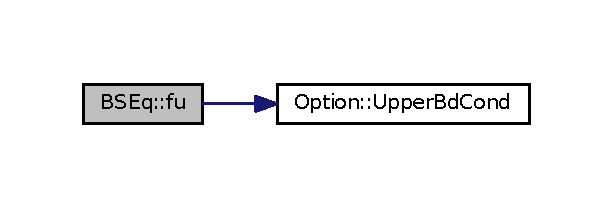
\includegraphics[width=294pt]{classBSEq_acebc22c41d04659861ef346d988de565_cgraph}
\end{center}
\end{figure}




\subsection{Member Data Documentation}
\hypertarget{classBSEq_a44b63f8349d8ab91a1fb8fc026cdf142}{\index{B\+S\+Eq@{B\+S\+Eq}!Ptr\+Model@{Ptr\+Model}}
\index{Ptr\+Model@{Ptr\+Model}!B\+S\+Eq@{B\+S\+Eq}}
\subsubsection[{Ptr\+Model}]{\setlength{\rightskip}{0pt plus 5cm}{\bf B\+S\+Model}$\ast$ B\+S\+Eq\+::\+Ptr\+Model}}\label{classBSEq_a44b63f8349d8ab91a1fb8fc026cdf142}


Definition at line \hyperlink{BSEq_8h_source_l00059}{59} of file \hyperlink{BSEq_8h_source}{B\+S\+Eq.\+h}.

\hypertarget{classBSEq_a280b15d8a4cd19d1aefc9feeb35a75bb}{\index{B\+S\+Eq@{B\+S\+Eq}!Ptr\+Option@{Ptr\+Option}}
\index{Ptr\+Option@{Ptr\+Option}!B\+S\+Eq@{B\+S\+Eq}}
\subsubsection[{Ptr\+Option}]{\setlength{\rightskip}{0pt plus 5cm}{\bf Option}$\ast$ B\+S\+Eq\+::\+Ptr\+Option}}\label{classBSEq_a280b15d8a4cd19d1aefc9feeb35a75bb}


Definition at line \hyperlink{BSEq_8h_source_l00060}{60} of file \hyperlink{BSEq_8h_source}{B\+S\+Eq.\+h}.



The documentation for this class was generated from the following files\+:\begin{DoxyCompactItemize}
\item 
\hyperlink{BSEq_8h}{B\+S\+Eq.\+h}\item 
\hyperlink{BSEq_8cpp}{B\+S\+Eq.\+cpp}\end{DoxyCompactItemize}

\hypertarget{classBSModel}{\section{B\+S\+Model Class Reference}
\label{classBSModel}\index{B\+S\+Model@{B\+S\+Model}}
}


{\ttfamily \#include $<$B\+S\+Model01.\+h$>$}



Collaboration diagram for B\+S\+Model\+:\nopagebreak
\begin{figure}[H]
\begin{center}
\leavevmode
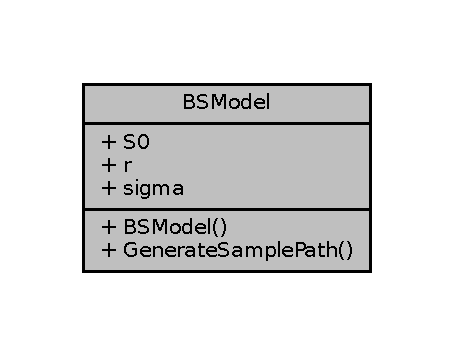
\includegraphics[width=218pt]{classBSModel__coll__graph}
\end{center}
\end{figure}
\subsection*{Public Member Functions}
\begin{DoxyCompactItemize}
\item 
\hyperlink{classBSModel_a309dd895251cfd050b2d50a30abfc5fb}{B\+S\+Model} (double S0\+\_\+, double r\+\_\+, double sigma\+\_\+)
\item 
void \hyperlink{classBSModel_aad0f0d6d1b9df4d76d03bd0b477e1347}{Generate\+Sample\+Path} (double T, int m, \hyperlink{BSModel01_8h_afbb1a5715857075c187084894fc00d31}{Sample\+Path} \&S)
\end{DoxyCompactItemize}
\subsection*{Public Attributes}
\begin{DoxyCompactItemize}
\item 
double \hyperlink{classBSModel_a2b37a14d9aaab033d676dd16381f7f19}{S0}
\item 
double \hyperlink{classBSModel_add3230c0df8e47623116b439598c0de3}{r}
\item 
double \hyperlink{classBSModel_a1267641043c16cd9baf2eb242320f0d3}{sigma}
\end{DoxyCompactItemize}


\subsection{Detailed Description}


Definition at line \hyperlink{BSModel01_8h_source_l00031}{31} of file \hyperlink{BSModel01_8h_source}{B\+S\+Model01.\+h}.



\subsection{Constructor \& Destructor Documentation}
\hypertarget{classBSModel_a309dd895251cfd050b2d50a30abfc5fb}{\index{B\+S\+Model@{B\+S\+Model}!B\+S\+Model@{B\+S\+Model}}
\index{B\+S\+Model@{B\+S\+Model}!B\+S\+Model@{B\+S\+Model}}
\subsubsection[{B\+S\+Model}]{\setlength{\rightskip}{0pt plus 5cm}B\+S\+Model\+::\+B\+S\+Model (
\begin{DoxyParamCaption}
\item[{double}]{S0\+\_\+, }
\item[{double}]{r\+\_\+, }
\item[{double}]{sigma\+\_\+}
\end{DoxyParamCaption}
)\hspace{0.3cm}{\ttfamily [inline]}}}\label{classBSModel_a309dd895251cfd050b2d50a30abfc5fb}


Definition at line \hyperlink{BSModel01_8h_source_l00037}{37} of file \hyperlink{BSModel01_8h_source}{B\+S\+Model01.\+h}.



\subsection{Member Function Documentation}
\hypertarget{classBSModel_aad0f0d6d1b9df4d76d03bd0b477e1347}{\index{B\+S\+Model@{B\+S\+Model}!Generate\+Sample\+Path@{Generate\+Sample\+Path}}
\index{Generate\+Sample\+Path@{Generate\+Sample\+Path}!B\+S\+Model@{B\+S\+Model}}
\subsubsection[{Generate\+Sample\+Path}]{\setlength{\rightskip}{0pt plus 5cm}void B\+S\+Model\+::\+Generate\+Sample\+Path (
\begin{DoxyParamCaption}
\item[{double}]{T, }
\item[{int}]{m, }
\item[{{\bf Sample\+Path} \&}]{S}
\end{DoxyParamCaption}
)}}\label{classBSModel_aad0f0d6d1b9df4d76d03bd0b477e1347}


Definition at line \hyperlink{BSModel01_8cpp_source_l00033}{33} of file \hyperlink{BSModel01_8cpp_source}{B\+S\+Model01.\+cpp}.



Here is the call graph for this function\+:\nopagebreak
\begin{figure}[H]
\begin{center}
\leavevmode
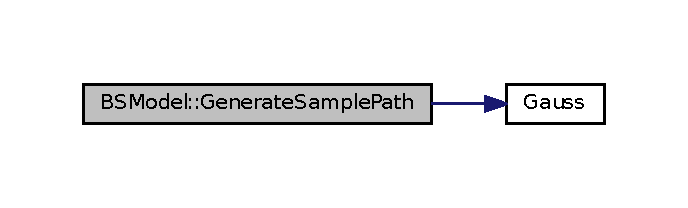
\includegraphics[width=330pt]{classBSModel_aad0f0d6d1b9df4d76d03bd0b477e1347_cgraph}
\end{center}
\end{figure}




\subsection{Member Data Documentation}
\hypertarget{classBSModel_add3230c0df8e47623116b439598c0de3}{\index{B\+S\+Model@{B\+S\+Model}!r@{r}}
\index{r@{r}!B\+S\+Model@{B\+S\+Model}}
\subsubsection[{r}]{\setlength{\rightskip}{0pt plus 5cm}double B\+S\+Model\+::r}}\label{classBSModel_add3230c0df8e47623116b439598c0de3}


Definition at line \hyperlink{BSModel01_8h_source_l00034}{34} of file \hyperlink{BSModel01_8h_source}{B\+S\+Model01.\+h}.

\hypertarget{classBSModel_a2b37a14d9aaab033d676dd16381f7f19}{\index{B\+S\+Model@{B\+S\+Model}!S0@{S0}}
\index{S0@{S0}!B\+S\+Model@{B\+S\+Model}}
\subsubsection[{S0}]{\setlength{\rightskip}{0pt plus 5cm}double B\+S\+Model\+::\+S0}}\label{classBSModel_a2b37a14d9aaab033d676dd16381f7f19}


Definition at line \hyperlink{BSModel01_8h_source_l00033}{33} of file \hyperlink{BSModel01_8h_source}{B\+S\+Model01.\+h}.

\hypertarget{classBSModel_a1267641043c16cd9baf2eb242320f0d3}{\index{B\+S\+Model@{B\+S\+Model}!sigma@{sigma}}
\index{sigma@{sigma}!B\+S\+Model@{B\+S\+Model}}
\subsubsection[{sigma}]{\setlength{\rightskip}{0pt plus 5cm}double B\+S\+Model\+::sigma}}\label{classBSModel_a1267641043c16cd9baf2eb242320f0d3}


Definition at line \hyperlink{BSModel01_8h_source_l00035}{35} of file \hyperlink{BSModel01_8h_source}{B\+S\+Model01.\+h}.



The documentation for this class was generated from the following files\+:\begin{DoxyCompactItemize}
\item 
\hyperlink{BSModel01_8h}{B\+S\+Model01.\+h}\item 
\hyperlink{BSModel01_8cpp}{B\+S\+Model01.\+cpp}\end{DoxyCompactItemize}

\hypertarget{classExplicitMethod}{\section{Explicit\+Method Class Reference}
\label{classExplicitMethod}\index{Explicit\+Method@{Explicit\+Method}}
}


{\ttfamily \#include $<$Explicit\+Method.\+h$>$}



Inheritance diagram for Explicit\+Method\+:\nopagebreak
\begin{figure}[H]
\begin{center}
\leavevmode
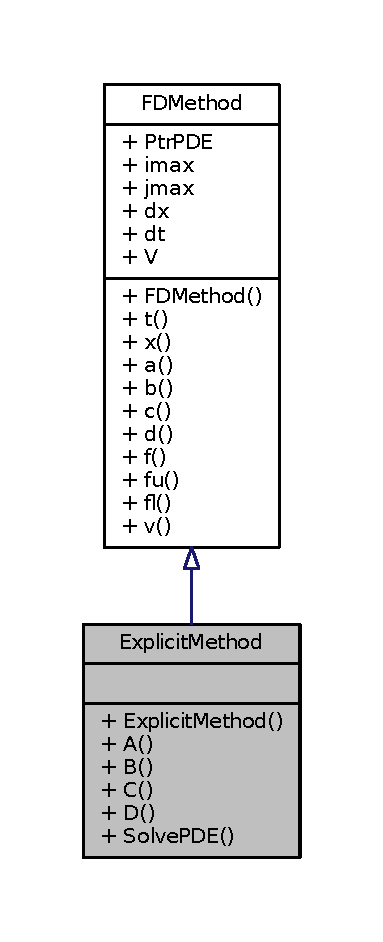
\includegraphics[width=184pt]{classExplicitMethod__inherit__graph}
\end{center}
\end{figure}


Collaboration diagram for Explicit\+Method\+:\nopagebreak
\begin{figure}[H]
\begin{center}
\leavevmode
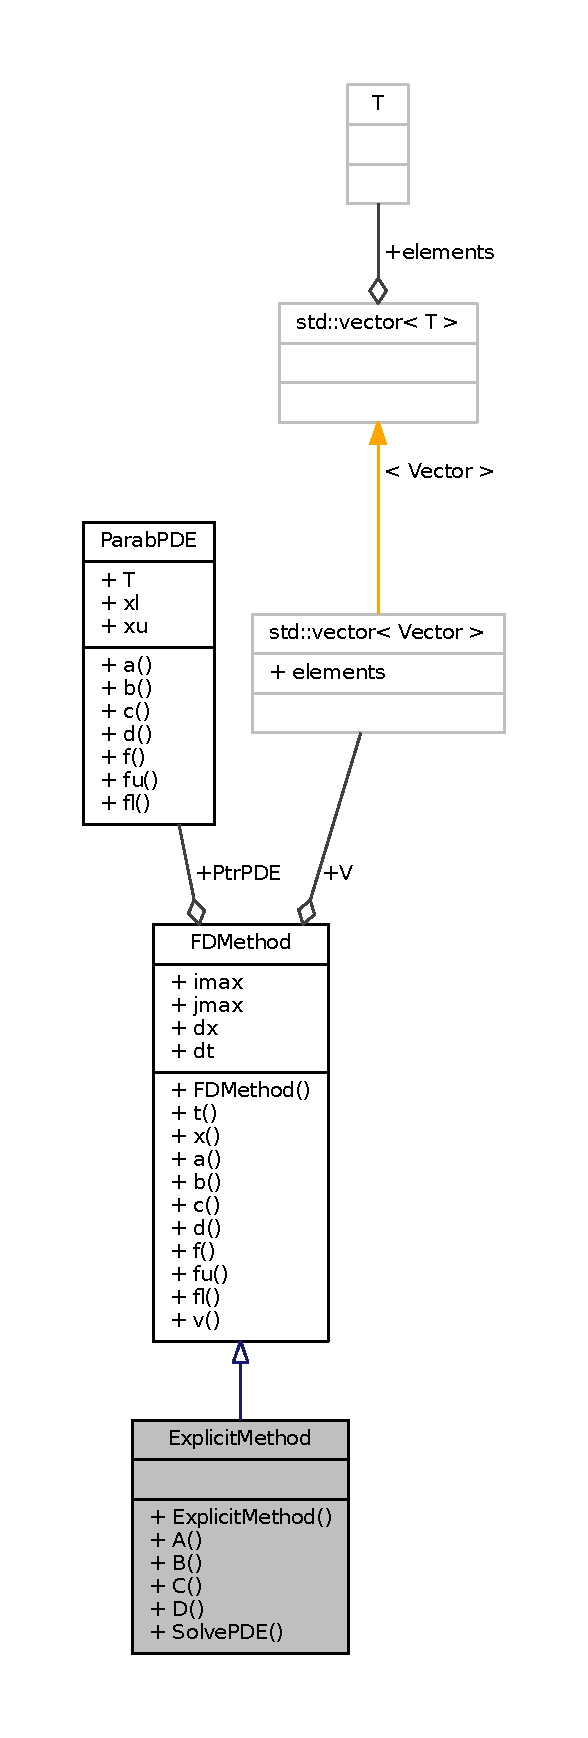
\includegraphics[height=550pt]{classExplicitMethod__coll__graph}
\end{center}
\end{figure}
\subsection*{Public Member Functions}
\begin{DoxyCompactItemize}
\item 
\hyperlink{classExplicitMethod_a49a9754a22eb54753173fc66c4a3d98b}{Explicit\+Method} (\hyperlink{classParabPDE}{Parab\+P\+D\+E} $\ast$Ptr\+P\+D\+E\+\_\+, int imax\+\_\+, int jmax\+\_\+)
\item 
double \hyperlink{classExplicitMethod_a82663c50a40a9877634499d65596e3da}{A} (int i, int j)
\item 
double \hyperlink{classExplicitMethod_a22b9be6bfd28ade5209422a47f6aa9c6}{B} (int i, int j)
\item 
double \hyperlink{classExplicitMethod_a857b126f5aee76df8fedff16ae506e52}{C} (int i, int j)
\item 
double \hyperlink{classExplicitMethod_af3dffe59f3c812828af74b0de39556cd}{D} (int i, int j)
\item 
void \hyperlink{classExplicitMethod_ac2c2d5bac3fc414851c2810ff916c2d6}{Solve\+P\+D\+E} ()
\end{DoxyCompactItemize}
\subsection*{Additional Inherited Members}


\subsection{Detailed Description}


Definition at line \hyperlink{ExplicitMethod_8h_source_l00006}{6} of file \hyperlink{ExplicitMethod_8h_source}{Explicit\+Method.\+h}.



\subsection{Constructor \& Destructor Documentation}
\hypertarget{classExplicitMethod_a49a9754a22eb54753173fc66c4a3d98b}{\index{Explicit\+Method@{Explicit\+Method}!Explicit\+Method@{Explicit\+Method}}
\index{Explicit\+Method@{Explicit\+Method}!Explicit\+Method@{Explicit\+Method}}
\subsubsection[{Explicit\+Method}]{\setlength{\rightskip}{0pt plus 5cm}Explicit\+Method\+::\+Explicit\+Method (
\begin{DoxyParamCaption}
\item[{{\bf Parab\+P\+D\+E} $\ast$}]{Ptr\+P\+D\+E\+\_\+, }
\item[{int}]{imax\+\_\+, }
\item[{int}]{jmax\+\_\+}
\end{DoxyParamCaption}
)\hspace{0.3cm}{\ttfamily [inline]}}}\label{classExplicitMethod_a49a9754a22eb54753173fc66c4a3d98b}


Definition at line \hyperlink{ExplicitMethod_8h_source_l00009}{9} of file \hyperlink{ExplicitMethod_8h_source}{Explicit\+Method.\+h}.



\subsection{Member Function Documentation}
\hypertarget{classExplicitMethod_a82663c50a40a9877634499d65596e3da}{\index{Explicit\+Method@{Explicit\+Method}!A@{A}}
\index{A@{A}!Explicit\+Method@{Explicit\+Method}}
\subsubsection[{A}]{\setlength{\rightskip}{0pt plus 5cm}double Explicit\+Method\+::\+A (
\begin{DoxyParamCaption}
\item[{int}]{i, }
\item[{int}]{j}
\end{DoxyParamCaption}
)\hspace{0.3cm}{\ttfamily [inline]}}}\label{classExplicitMethod_a82663c50a40a9877634499d65596e3da}


Definition at line \hyperlink{ExplicitMethod_8h_source_l00012}{12} of file \hyperlink{ExplicitMethod_8h_source}{Explicit\+Method.\+h}.



Here is the call graph for this function\+:\nopagebreak
\begin{figure}[H]
\begin{center}
\leavevmode
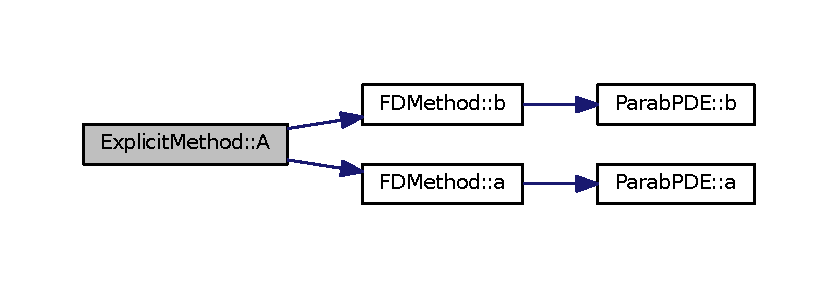
\includegraphics[width=350pt]{classExplicitMethod_a82663c50a40a9877634499d65596e3da_cgraph}
\end{center}
\end{figure}




Here is the caller graph for this function\+:\nopagebreak
\begin{figure}[H]
\begin{center}
\leavevmode
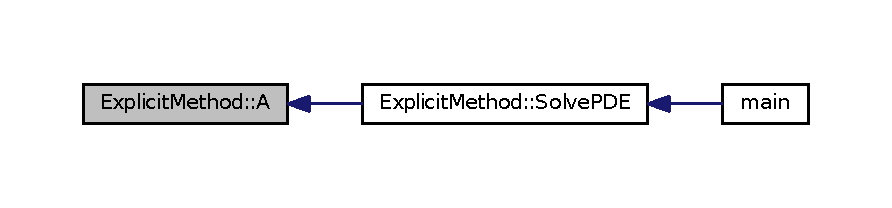
\includegraphics[width=350pt]{classExplicitMethod_a82663c50a40a9877634499d65596e3da_icgraph}
\end{center}
\end{figure}


\hypertarget{classExplicitMethod_a22b9be6bfd28ade5209422a47f6aa9c6}{\index{Explicit\+Method@{Explicit\+Method}!B@{B}}
\index{B@{B}!Explicit\+Method@{Explicit\+Method}}
\subsubsection[{B}]{\setlength{\rightskip}{0pt plus 5cm}double Explicit\+Method\+::\+B (
\begin{DoxyParamCaption}
\item[{int}]{i, }
\item[{int}]{j}
\end{DoxyParamCaption}
)\hspace{0.3cm}{\ttfamily [inline]}}}\label{classExplicitMethod_a22b9be6bfd28ade5209422a47f6aa9c6}


Definition at line \hyperlink{ExplicitMethod_8h_source_l00015}{15} of file \hyperlink{ExplicitMethod_8h_source}{Explicit\+Method.\+h}.



Here is the call graph for this function\+:\nopagebreak
\begin{figure}[H]
\begin{center}
\leavevmode
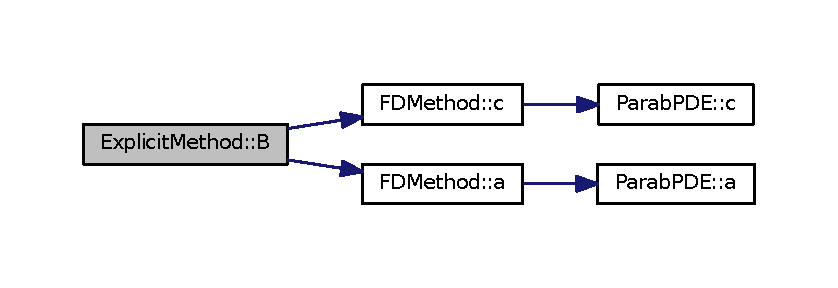
\includegraphics[width=350pt]{classExplicitMethod_a22b9be6bfd28ade5209422a47f6aa9c6_cgraph}
\end{center}
\end{figure}




Here is the caller graph for this function\+:\nopagebreak
\begin{figure}[H]
\begin{center}
\leavevmode
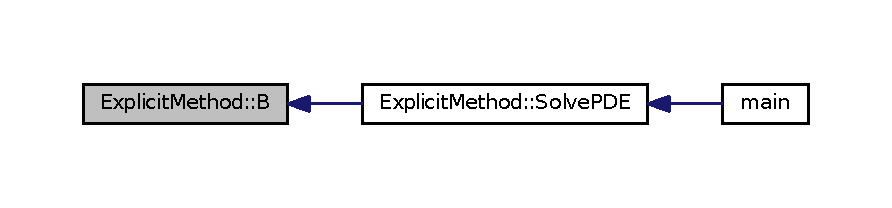
\includegraphics[width=350pt]{classExplicitMethod_a22b9be6bfd28ade5209422a47f6aa9c6_icgraph}
\end{center}
\end{figure}


\hypertarget{classExplicitMethod_a857b126f5aee76df8fedff16ae506e52}{\index{Explicit\+Method@{Explicit\+Method}!C@{C}}
\index{C@{C}!Explicit\+Method@{Explicit\+Method}}
\subsubsection[{C}]{\setlength{\rightskip}{0pt plus 5cm}double Explicit\+Method\+::\+C (
\begin{DoxyParamCaption}
\item[{int}]{i, }
\item[{int}]{j}
\end{DoxyParamCaption}
)\hspace{0.3cm}{\ttfamily [inline]}}}\label{classExplicitMethod_a857b126f5aee76df8fedff16ae506e52}


Definition at line \hyperlink{ExplicitMethod_8h_source_l00018}{18} of file \hyperlink{ExplicitMethod_8h_source}{Explicit\+Method.\+h}.



Here is the call graph for this function\+:\nopagebreak
\begin{figure}[H]
\begin{center}
\leavevmode
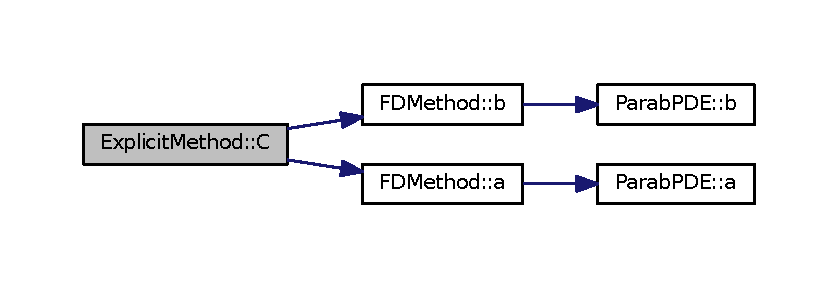
\includegraphics[width=350pt]{classExplicitMethod_a857b126f5aee76df8fedff16ae506e52_cgraph}
\end{center}
\end{figure}




Here is the caller graph for this function\+:\nopagebreak
\begin{figure}[H]
\begin{center}
\leavevmode
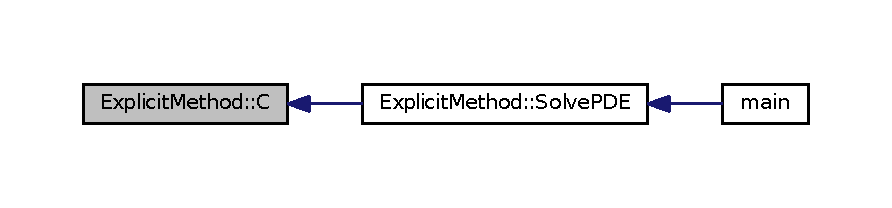
\includegraphics[width=350pt]{classExplicitMethod_a857b126f5aee76df8fedff16ae506e52_icgraph}
\end{center}
\end{figure}


\hypertarget{classExplicitMethod_af3dffe59f3c812828af74b0de39556cd}{\index{Explicit\+Method@{Explicit\+Method}!D@{D}}
\index{D@{D}!Explicit\+Method@{Explicit\+Method}}
\subsubsection[{D}]{\setlength{\rightskip}{0pt plus 5cm}double Explicit\+Method\+::\+D (
\begin{DoxyParamCaption}
\item[{int}]{i, }
\item[{int}]{j}
\end{DoxyParamCaption}
)\hspace{0.3cm}{\ttfamily [inline]}}}\label{classExplicitMethod_af3dffe59f3c812828af74b0de39556cd}


Definition at line \hyperlink{ExplicitMethod_8h_source_l00021}{21} of file \hyperlink{ExplicitMethod_8h_source}{Explicit\+Method.\+h}.



Here is the call graph for this function\+:\nopagebreak
\begin{figure}[H]
\begin{center}
\leavevmode
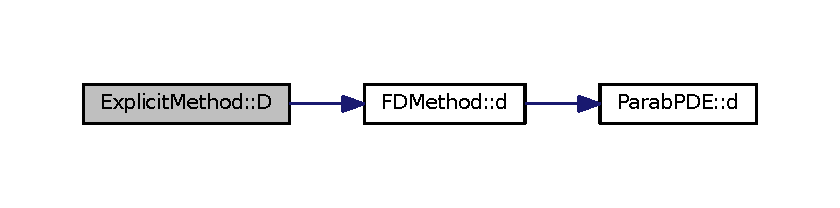
\includegraphics[width=350pt]{classExplicitMethod_af3dffe59f3c812828af74b0de39556cd_cgraph}
\end{center}
\end{figure}




Here is the caller graph for this function\+:\nopagebreak
\begin{figure}[H]
\begin{center}
\leavevmode
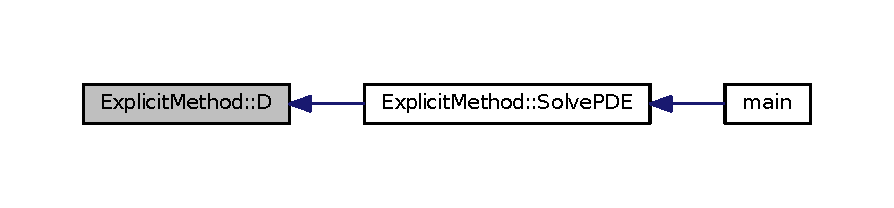
\includegraphics[width=350pt]{classExplicitMethod_af3dffe59f3c812828af74b0de39556cd_icgraph}
\end{center}
\end{figure}


\hypertarget{classExplicitMethod_ac2c2d5bac3fc414851c2810ff916c2d6}{\index{Explicit\+Method@{Explicit\+Method}!Solve\+P\+D\+E@{Solve\+P\+D\+E}}
\index{Solve\+P\+D\+E@{Solve\+P\+D\+E}!Explicit\+Method@{Explicit\+Method}}
\subsubsection[{Solve\+P\+D\+E}]{\setlength{\rightskip}{0pt plus 5cm}void Explicit\+Method\+::\+Solve\+P\+D\+E (
\begin{DoxyParamCaption}
{}
\end{DoxyParamCaption}
)}}\label{classExplicitMethod_ac2c2d5bac3fc414851c2810ff916c2d6}


Definition at line \hyperlink{ExplicitMethod_8cpp_source_l00003}{3} of file \hyperlink{ExplicitMethod_8cpp_source}{Explicit\+Method.\+cpp}.



Here is the call graph for this function\+:\nopagebreak
\begin{figure}[H]
\begin{center}
\leavevmode
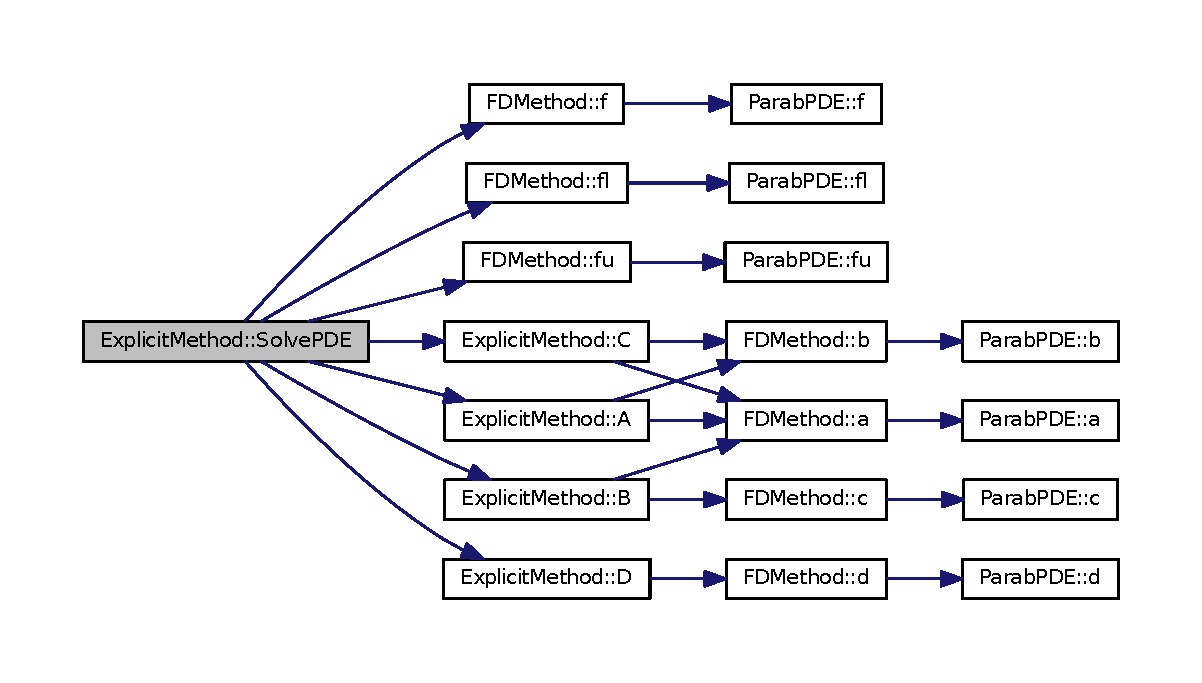
\includegraphics[width=350pt]{classExplicitMethod_ac2c2d5bac3fc414851c2810ff916c2d6_cgraph}
\end{center}
\end{figure}




Here is the caller graph for this function\+:\nopagebreak
\begin{figure}[H]
\begin{center}
\leavevmode
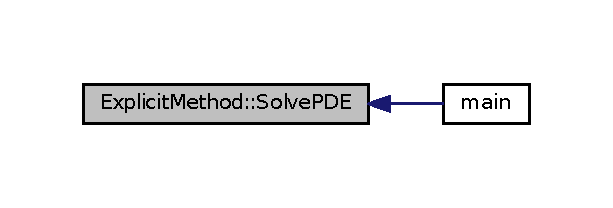
\includegraphics[width=294pt]{classExplicitMethod_ac2c2d5bac3fc414851c2810ff916c2d6_icgraph}
\end{center}
\end{figure}




The documentation for this class was generated from the following files\+:\begin{DoxyCompactItemize}
\item 
\hyperlink{ExplicitMethod_8h}{Explicit\+Method.\+h}\item 
\hyperlink{ExplicitMethod_8cpp}{Explicit\+Method.\+cpp}\end{DoxyCompactItemize}

\hypertarget{classFDMethod}{\section{F\+D\+Method Class Reference}
\label{classFDMethod}\index{F\+D\+Method@{F\+D\+Method}}
}


{\ttfamily \#include $<$F\+D\+Method.\+h$>$}



Inheritance diagram for F\+D\+Method\+:\nopagebreak
\begin{figure}[H]
\begin{center}
\leavevmode
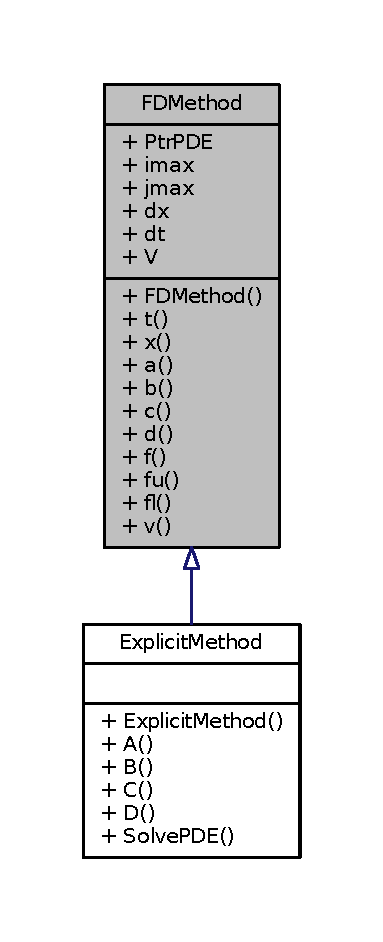
\includegraphics[width=184pt]{classFDMethod__inherit__graph}
\end{center}
\end{figure}


Collaboration diagram for F\+D\+Method\+:\nopagebreak
\begin{figure}[H]
\begin{center}
\leavevmode
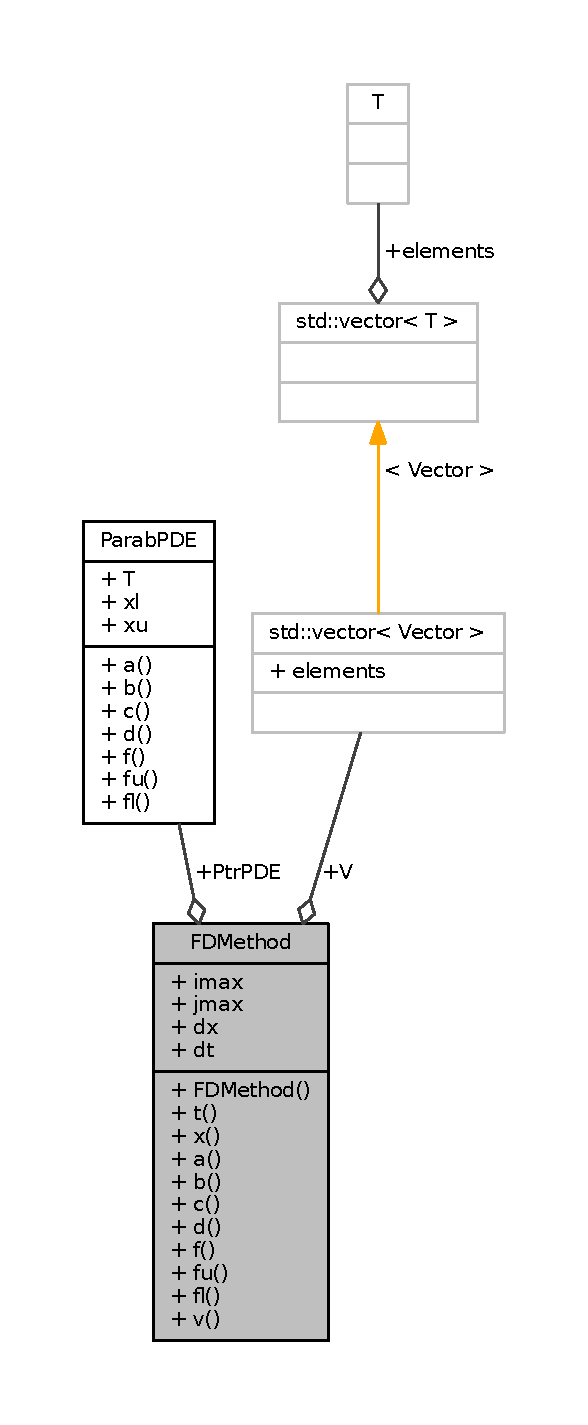
\includegraphics[height=550pt]{classFDMethod__coll__graph}
\end{center}
\end{figure}
\subsection*{Public Member Functions}
\begin{DoxyCompactItemize}
\item 
\hyperlink{classFDMethod_a87a98e06038c3bc9e88e639ded56d1cb}{F\+D\+Method} (\hyperlink{classParabPDE}{Parab\+P\+D\+E} $\ast$Ptr\+P\+D\+E\+\_\+, int imax\+\_\+, int jmax\+\_\+)
\item 
double \hyperlink{classFDMethod_a9aaf3e419045497b888808537fef2b19}{t} (double i)
\item 
double \hyperlink{classFDMethod_a8e5c9b6b56eb6c9d00267a4028814314}{x} (int j)
\item 
double \hyperlink{classFDMethod_a2b5d6d1d62048312725c60c5a99ee0d1}{a} (double i, int j)
\item 
double \hyperlink{classFDMethod_a50c258eaca61c1ed34247ad827379668}{b} (double i, int j)
\item 
double \hyperlink{classFDMethod_ad5c8725fb0379fa8cb29bb0954d60112}{c} (double i, int j)
\item 
double \hyperlink{classFDMethod_a4ad2213e6338bdfc2cc8a2b4e7eb0952}{d} (double i, int j)
\item 
double \hyperlink{classFDMethod_a02f9d3f5c3466f04323bb966b346efae}{f} (int j)
\item 
double \hyperlink{classFDMethod_ae282bd4b389fdce1badb5ecaa3c3e8e5}{fu} (int i)
\item 
double \hyperlink{classFDMethod_add9102baa92871331350bf5d86c12f1a}{fl} (int i)
\item 
double \hyperlink{classFDMethod_a703b25f3d7f5083bfd9fbbe9e1906946}{v} (double \hyperlink{classFDMethod_a9aaf3e419045497b888808537fef2b19}{t}, double \hyperlink{classFDMethod_a8e5c9b6b56eb6c9d00267a4028814314}{x})
\end{DoxyCompactItemize}
\subsection*{Public Attributes}
\begin{DoxyCompactItemize}
\item 
\hyperlink{classParabPDE}{Parab\+P\+D\+E} $\ast$ \hyperlink{classFDMethod_a900e2425569c70cf67c0b89fbeb15aba}{Ptr\+P\+D\+E}
\item 
int \hyperlink{classFDMethod_a72f22ed3e70c7f6084d3499fa7fbad38}{imax}
\item 
int \hyperlink{classFDMethod_a6d4cec47464758c00c5d65cfa676d518}{jmax}
\item 
double \hyperlink{classFDMethod_aec2698863360e900a8d84f7d672484c9}{dx}
\item 
double \hyperlink{classFDMethod_a4748bd052a59842154022b9aa6b55737}{dt}
\item 
vector$<$ \hyperlink{FDMethod_8h_a9a0795b74fd145527f628932c8884ffe}{Vector} $>$ \hyperlink{classFDMethod_a627ca1e8a18af23dbbe44a43cbc2831e}{V}
\end{DoxyCompactItemize}


\subsection{Detailed Description}


Definition at line \hyperlink{FDMethod_8h_source_l00012}{12} of file \hyperlink{FDMethod_8h_source}{F\+D\+Method.\+h}.



\subsection{Constructor \& Destructor Documentation}
\hypertarget{classFDMethod_a87a98e06038c3bc9e88e639ded56d1cb}{\index{F\+D\+Method@{F\+D\+Method}!F\+D\+Method@{F\+D\+Method}}
\index{F\+D\+Method@{F\+D\+Method}!F\+D\+Method@{F\+D\+Method}}
\subsubsection[{F\+D\+Method}]{\setlength{\rightskip}{0pt plus 5cm}F\+D\+Method\+::\+F\+D\+Method (
\begin{DoxyParamCaption}
\item[{{\bf Parab\+P\+D\+E} $\ast$}]{Ptr\+P\+D\+E\+\_\+, }
\item[{int}]{imax\+\_\+, }
\item[{int}]{jmax\+\_\+}
\end{DoxyParamCaption}
)}}\label{classFDMethod_a87a98e06038c3bc9e88e639ded56d1cb}


Definition at line \hyperlink{FDMethod_8cpp_source_l00003}{3} of file \hyperlink{FDMethod_8cpp_source}{F\+D\+Method.\+cpp}.



\subsection{Member Function Documentation}
\hypertarget{classFDMethod_a2b5d6d1d62048312725c60c5a99ee0d1}{\index{F\+D\+Method@{F\+D\+Method}!a@{a}}
\index{a@{a}!F\+D\+Method@{F\+D\+Method}}
\subsubsection[{a}]{\setlength{\rightskip}{0pt plus 5cm}double F\+D\+Method\+::a (
\begin{DoxyParamCaption}
\item[{double}]{i, }
\item[{int}]{j}
\end{DoxyParamCaption}
)\hspace{0.3cm}{\ttfamily [inline]}}}\label{classFDMethod_a2b5d6d1d62048312725c60c5a99ee0d1}


Definition at line \hyperlink{FDMethod_8h_source_l00029}{29} of file \hyperlink{FDMethod_8h_source}{F\+D\+Method.\+h}.



Here is the call graph for this function\+:\nopagebreak
\begin{figure}[H]
\begin{center}
\leavevmode
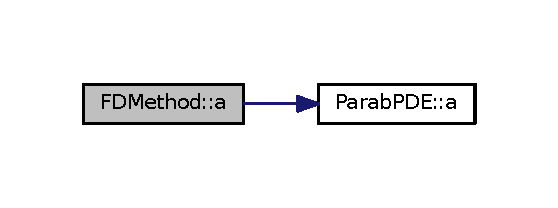
\includegraphics[width=268pt]{classFDMethod_a2b5d6d1d62048312725c60c5a99ee0d1_cgraph}
\end{center}
\end{figure}




Here is the caller graph for this function\+:\nopagebreak
\begin{figure}[H]
\begin{center}
\leavevmode
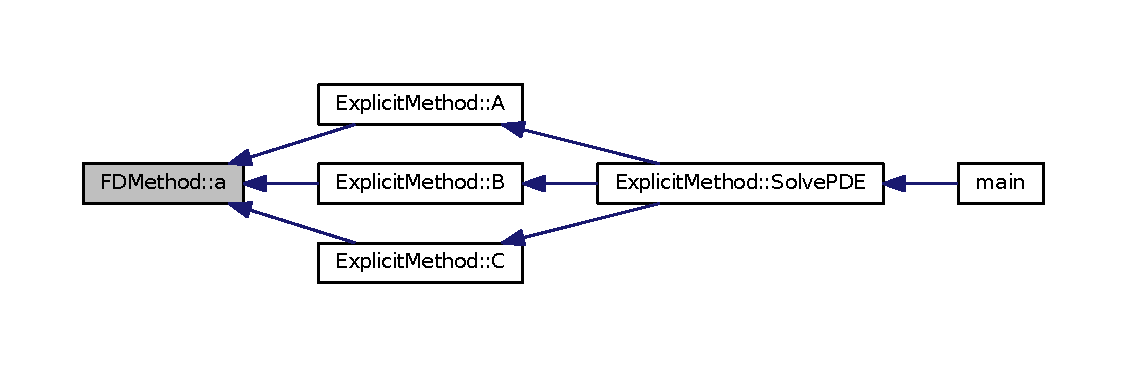
\includegraphics[width=350pt]{classFDMethod_a2b5d6d1d62048312725c60c5a99ee0d1_icgraph}
\end{center}
\end{figure}


\hypertarget{classFDMethod_a50c258eaca61c1ed34247ad827379668}{\index{F\+D\+Method@{F\+D\+Method}!b@{b}}
\index{b@{b}!F\+D\+Method@{F\+D\+Method}}
\subsubsection[{b}]{\setlength{\rightskip}{0pt plus 5cm}double F\+D\+Method\+::b (
\begin{DoxyParamCaption}
\item[{double}]{i, }
\item[{int}]{j}
\end{DoxyParamCaption}
)\hspace{0.3cm}{\ttfamily [inline]}}}\label{classFDMethod_a50c258eaca61c1ed34247ad827379668}


Definition at line \hyperlink{FDMethod_8h_source_l00032}{32} of file \hyperlink{FDMethod_8h_source}{F\+D\+Method.\+h}.



Here is the call graph for this function\+:\nopagebreak
\begin{figure}[H]
\begin{center}
\leavevmode
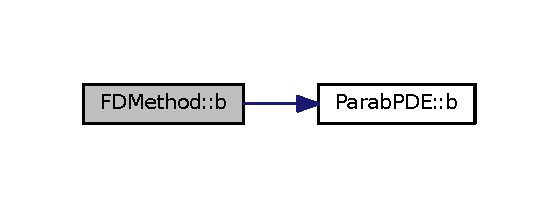
\includegraphics[width=268pt]{classFDMethod_a50c258eaca61c1ed34247ad827379668_cgraph}
\end{center}
\end{figure}




Here is the caller graph for this function\+:\nopagebreak
\begin{figure}[H]
\begin{center}
\leavevmode
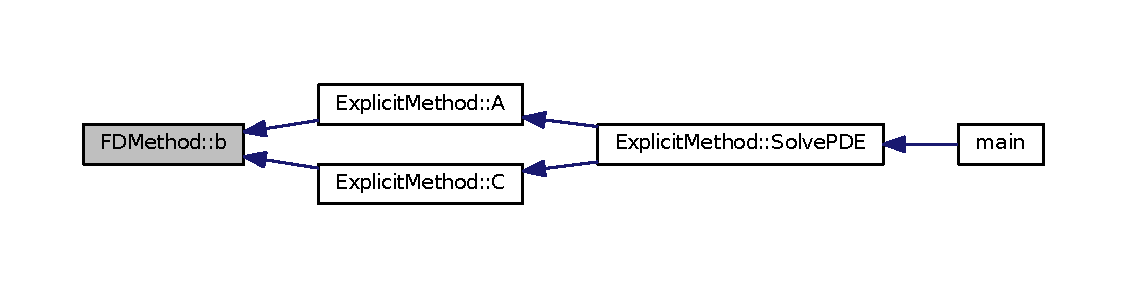
\includegraphics[width=350pt]{classFDMethod_a50c258eaca61c1ed34247ad827379668_icgraph}
\end{center}
\end{figure}


\hypertarget{classFDMethod_ad5c8725fb0379fa8cb29bb0954d60112}{\index{F\+D\+Method@{F\+D\+Method}!c@{c}}
\index{c@{c}!F\+D\+Method@{F\+D\+Method}}
\subsubsection[{c}]{\setlength{\rightskip}{0pt plus 5cm}double F\+D\+Method\+::c (
\begin{DoxyParamCaption}
\item[{double}]{i, }
\item[{int}]{j}
\end{DoxyParamCaption}
)\hspace{0.3cm}{\ttfamily [inline]}}}\label{classFDMethod_ad5c8725fb0379fa8cb29bb0954d60112}


Definition at line \hyperlink{FDMethod_8h_source_l00035}{35} of file \hyperlink{FDMethod_8h_source}{F\+D\+Method.\+h}.



Here is the call graph for this function\+:\nopagebreak
\begin{figure}[H]
\begin{center}
\leavevmode
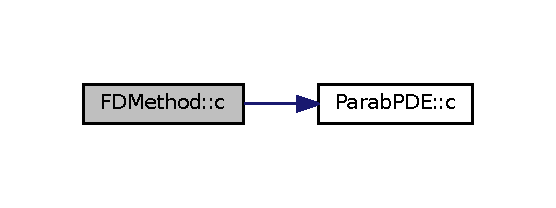
\includegraphics[width=267pt]{classFDMethod_ad5c8725fb0379fa8cb29bb0954d60112_cgraph}
\end{center}
\end{figure}




Here is the caller graph for this function\+:\nopagebreak
\begin{figure}[H]
\begin{center}
\leavevmode
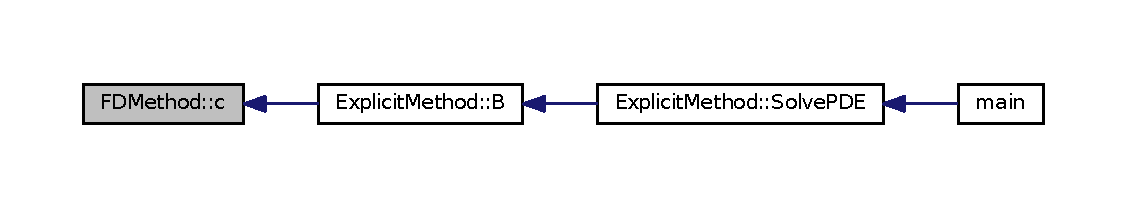
\includegraphics[width=350pt]{classFDMethod_ad5c8725fb0379fa8cb29bb0954d60112_icgraph}
\end{center}
\end{figure}


\hypertarget{classFDMethod_a4ad2213e6338bdfc2cc8a2b4e7eb0952}{\index{F\+D\+Method@{F\+D\+Method}!d@{d}}
\index{d@{d}!F\+D\+Method@{F\+D\+Method}}
\subsubsection[{d}]{\setlength{\rightskip}{0pt plus 5cm}double F\+D\+Method\+::d (
\begin{DoxyParamCaption}
\item[{double}]{i, }
\item[{int}]{j}
\end{DoxyParamCaption}
)\hspace{0.3cm}{\ttfamily [inline]}}}\label{classFDMethod_a4ad2213e6338bdfc2cc8a2b4e7eb0952}


Definition at line \hyperlink{FDMethod_8h_source_l00038}{38} of file \hyperlink{FDMethod_8h_source}{F\+D\+Method.\+h}.



Here is the call graph for this function\+:\nopagebreak
\begin{figure}[H]
\begin{center}
\leavevmode
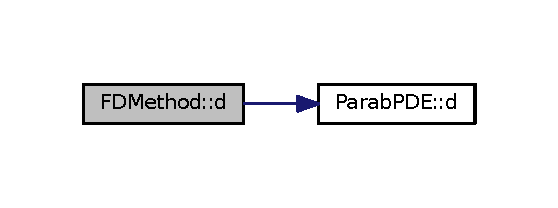
\includegraphics[width=268pt]{classFDMethod_a4ad2213e6338bdfc2cc8a2b4e7eb0952_cgraph}
\end{center}
\end{figure}




Here is the caller graph for this function\+:\nopagebreak
\begin{figure}[H]
\begin{center}
\leavevmode
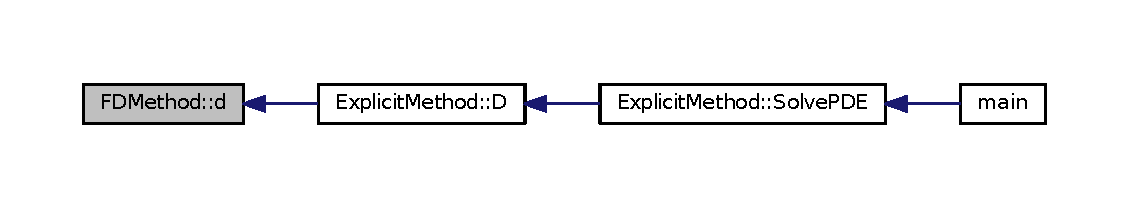
\includegraphics[width=350pt]{classFDMethod_a4ad2213e6338bdfc2cc8a2b4e7eb0952_icgraph}
\end{center}
\end{figure}


\hypertarget{classFDMethod_a02f9d3f5c3466f04323bb966b346efae}{\index{F\+D\+Method@{F\+D\+Method}!f@{f}}
\index{f@{f}!F\+D\+Method@{F\+D\+Method}}
\subsubsection[{f}]{\setlength{\rightskip}{0pt plus 5cm}double F\+D\+Method\+::f (
\begin{DoxyParamCaption}
\item[{int}]{j}
\end{DoxyParamCaption}
)\hspace{0.3cm}{\ttfamily [inline]}}}\label{classFDMethod_a02f9d3f5c3466f04323bb966b346efae}


Definition at line \hyperlink{FDMethod_8h_source_l00041}{41} of file \hyperlink{FDMethod_8h_source}{F\+D\+Method.\+h}.



Here is the call graph for this function\+:\nopagebreak
\begin{figure}[H]
\begin{center}
\leavevmode
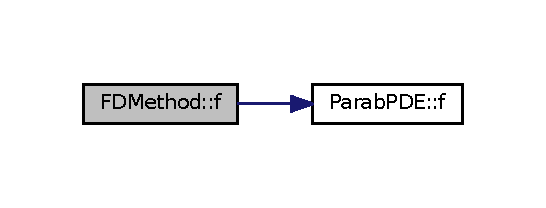
\includegraphics[width=262pt]{classFDMethod_a02f9d3f5c3466f04323bb966b346efae_cgraph}
\end{center}
\end{figure}




Here is the caller graph for this function\+:\nopagebreak
\begin{figure}[H]
\begin{center}
\leavevmode
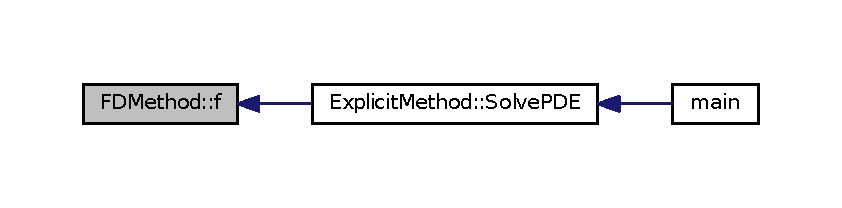
\includegraphics[width=350pt]{classFDMethod_a02f9d3f5c3466f04323bb966b346efae_icgraph}
\end{center}
\end{figure}


\hypertarget{classFDMethod_add9102baa92871331350bf5d86c12f1a}{\index{F\+D\+Method@{F\+D\+Method}!fl@{fl}}
\index{fl@{fl}!F\+D\+Method@{F\+D\+Method}}
\subsubsection[{fl}]{\setlength{\rightskip}{0pt plus 5cm}double F\+D\+Method\+::fl (
\begin{DoxyParamCaption}
\item[{int}]{i}
\end{DoxyParamCaption}
)\hspace{0.3cm}{\ttfamily [inline]}}}\label{classFDMethod_add9102baa92871331350bf5d86c12f1a}


Definition at line \hyperlink{FDMethod_8h_source_l00047}{47} of file \hyperlink{FDMethod_8h_source}{F\+D\+Method.\+h}.



Here is the call graph for this function\+:\nopagebreak
\begin{figure}[H]
\begin{center}
\leavevmode
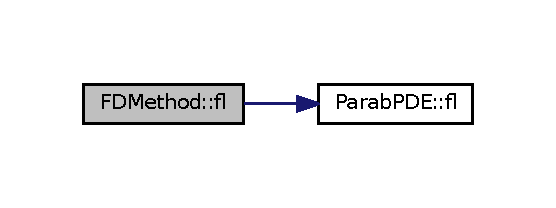
\includegraphics[width=267pt]{classFDMethod_add9102baa92871331350bf5d86c12f1a_cgraph}
\end{center}
\end{figure}




Here is the caller graph for this function\+:\nopagebreak
\begin{figure}[H]
\begin{center}
\leavevmode
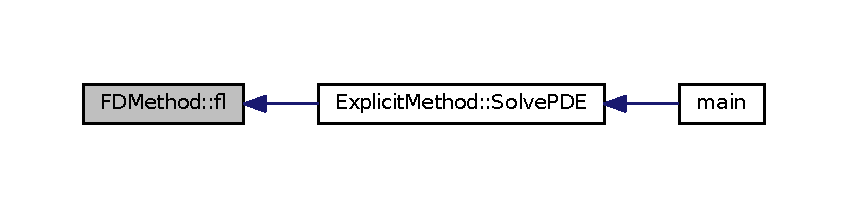
\includegraphics[width=350pt]{classFDMethod_add9102baa92871331350bf5d86c12f1a_icgraph}
\end{center}
\end{figure}


\hypertarget{classFDMethod_ae282bd4b389fdce1badb5ecaa3c3e8e5}{\index{F\+D\+Method@{F\+D\+Method}!fu@{fu}}
\index{fu@{fu}!F\+D\+Method@{F\+D\+Method}}
\subsubsection[{fu}]{\setlength{\rightskip}{0pt plus 5cm}double F\+D\+Method\+::fu (
\begin{DoxyParamCaption}
\item[{int}]{i}
\end{DoxyParamCaption}
)\hspace{0.3cm}{\ttfamily [inline]}}}\label{classFDMethod_ae282bd4b389fdce1badb5ecaa3c3e8e5}


Definition at line \hyperlink{FDMethod_8h_source_l00044}{44} of file \hyperlink{FDMethod_8h_source}{F\+D\+Method.\+h}.



Here is the call graph for this function\+:\nopagebreak
\begin{figure}[H]
\begin{center}
\leavevmode
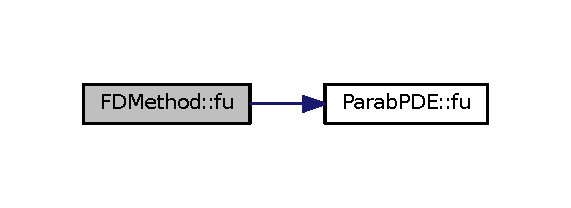
\includegraphics[width=274pt]{classFDMethod_ae282bd4b389fdce1badb5ecaa3c3e8e5_cgraph}
\end{center}
\end{figure}




Here is the caller graph for this function\+:\nopagebreak
\begin{figure}[H]
\begin{center}
\leavevmode
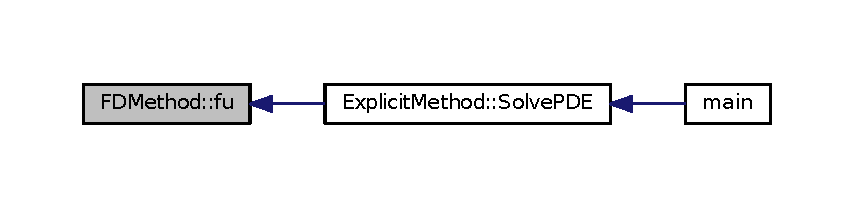
\includegraphics[width=350pt]{classFDMethod_ae282bd4b389fdce1badb5ecaa3c3e8e5_icgraph}
\end{center}
\end{figure}


\hypertarget{classFDMethod_a9aaf3e419045497b888808537fef2b19}{\index{F\+D\+Method@{F\+D\+Method}!t@{t}}
\index{t@{t}!F\+D\+Method@{F\+D\+Method}}
\subsubsection[{t}]{\setlength{\rightskip}{0pt plus 5cm}double F\+D\+Method\+::t (
\begin{DoxyParamCaption}
\item[{double}]{i}
\end{DoxyParamCaption}
)\hspace{0.3cm}{\ttfamily [inline]}}}\label{classFDMethod_a9aaf3e419045497b888808537fef2b19}


Definition at line \hyperlink{FDMethod_8h_source_l00023}{23} of file \hyperlink{FDMethod_8h_source}{F\+D\+Method.\+h}.



Here is the caller graph for this function\+:\nopagebreak
\begin{figure}[H]
\begin{center}
\leavevmode
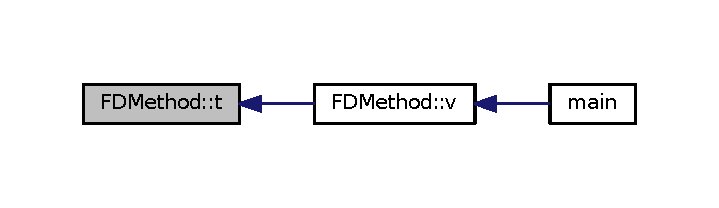
\includegraphics[width=345pt]{classFDMethod_a9aaf3e419045497b888808537fef2b19_icgraph}
\end{center}
\end{figure}


\hypertarget{classFDMethod_a703b25f3d7f5083bfd9fbbe9e1906946}{\index{F\+D\+Method@{F\+D\+Method}!v@{v}}
\index{v@{v}!F\+D\+Method@{F\+D\+Method}}
\subsubsection[{v}]{\setlength{\rightskip}{0pt plus 5cm}double F\+D\+Method\+::v (
\begin{DoxyParamCaption}
\item[{double}]{t, }
\item[{double}]{x}
\end{DoxyParamCaption}
)}}\label{classFDMethod_a703b25f3d7f5083bfd9fbbe9e1906946}


Definition at line \hyperlink{FDMethod_8cpp_source_l00017}{17} of file \hyperlink{FDMethod_8cpp_source}{F\+D\+Method.\+cpp}.



Here is the call graph for this function\+:\nopagebreak
\begin{figure}[H]
\begin{center}
\leavevmode
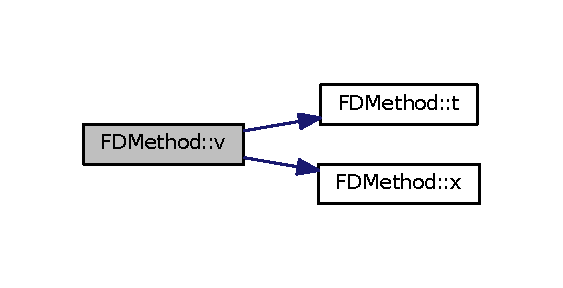
\includegraphics[width=270pt]{classFDMethod_a703b25f3d7f5083bfd9fbbe9e1906946_cgraph}
\end{center}
\end{figure}




Here is the caller graph for this function\+:\nopagebreak
\begin{figure}[H]
\begin{center}
\leavevmode
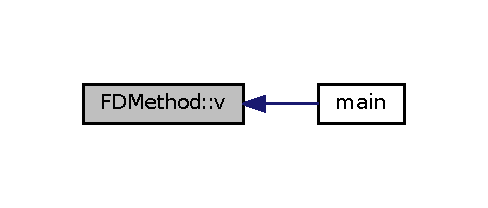
\includegraphics[width=234pt]{classFDMethod_a703b25f3d7f5083bfd9fbbe9e1906946_icgraph}
\end{center}
\end{figure}


\hypertarget{classFDMethod_a8e5c9b6b56eb6c9d00267a4028814314}{\index{F\+D\+Method@{F\+D\+Method}!x@{x}}
\index{x@{x}!F\+D\+Method@{F\+D\+Method}}
\subsubsection[{x}]{\setlength{\rightskip}{0pt plus 5cm}double F\+D\+Method\+::x (
\begin{DoxyParamCaption}
\item[{int}]{j}
\end{DoxyParamCaption}
)\hspace{0.3cm}{\ttfamily [inline]}}}\label{classFDMethod_a8e5c9b6b56eb6c9d00267a4028814314}


Definition at line \hyperlink{FDMethod_8h_source_l00026}{26} of file \hyperlink{FDMethod_8h_source}{F\+D\+Method.\+h}.



Here is the caller graph for this function\+:\nopagebreak
\begin{figure}[H]
\begin{center}
\leavevmode
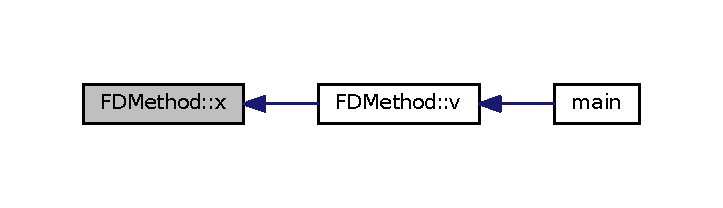
\includegraphics[width=347pt]{classFDMethod_a8e5c9b6b56eb6c9d00267a4028814314_icgraph}
\end{center}
\end{figure}




\subsection{Member Data Documentation}
\hypertarget{classFDMethod_a4748bd052a59842154022b9aa6b55737}{\index{F\+D\+Method@{F\+D\+Method}!dt@{dt}}
\index{dt@{dt}!F\+D\+Method@{F\+D\+Method}}
\subsubsection[{dt}]{\setlength{\rightskip}{0pt plus 5cm}double F\+D\+Method\+::dt}}\label{classFDMethod_a4748bd052a59842154022b9aa6b55737}


Definition at line \hyperlink{FDMethod_8h_source_l00018}{18} of file \hyperlink{FDMethod_8h_source}{F\+D\+Method.\+h}.

\hypertarget{classFDMethod_aec2698863360e900a8d84f7d672484c9}{\index{F\+D\+Method@{F\+D\+Method}!dx@{dx}}
\index{dx@{dx}!F\+D\+Method@{F\+D\+Method}}
\subsubsection[{dx}]{\setlength{\rightskip}{0pt plus 5cm}double F\+D\+Method\+::dx}}\label{classFDMethod_aec2698863360e900a8d84f7d672484c9}


Definition at line \hyperlink{FDMethod_8h_source_l00017}{17} of file \hyperlink{FDMethod_8h_source}{F\+D\+Method.\+h}.

\hypertarget{classFDMethod_a72f22ed3e70c7f6084d3499fa7fbad38}{\index{F\+D\+Method@{F\+D\+Method}!imax@{imax}}
\index{imax@{imax}!F\+D\+Method@{F\+D\+Method}}
\subsubsection[{imax}]{\setlength{\rightskip}{0pt plus 5cm}int F\+D\+Method\+::imax}}\label{classFDMethod_a72f22ed3e70c7f6084d3499fa7fbad38}


Definition at line \hyperlink{FDMethod_8h_source_l00015}{15} of file \hyperlink{FDMethod_8h_source}{F\+D\+Method.\+h}.

\hypertarget{classFDMethod_a6d4cec47464758c00c5d65cfa676d518}{\index{F\+D\+Method@{F\+D\+Method}!jmax@{jmax}}
\index{jmax@{jmax}!F\+D\+Method@{F\+D\+Method}}
\subsubsection[{jmax}]{\setlength{\rightskip}{0pt plus 5cm}int F\+D\+Method\+::jmax}}\label{classFDMethod_a6d4cec47464758c00c5d65cfa676d518}


Definition at line \hyperlink{FDMethod_8h_source_l00016}{16} of file \hyperlink{FDMethod_8h_source}{F\+D\+Method.\+h}.

\hypertarget{classFDMethod_a900e2425569c70cf67c0b89fbeb15aba}{\index{F\+D\+Method@{F\+D\+Method}!Ptr\+P\+D\+E@{Ptr\+P\+D\+E}}
\index{Ptr\+P\+D\+E@{Ptr\+P\+D\+E}!F\+D\+Method@{F\+D\+Method}}
\subsubsection[{Ptr\+P\+D\+E}]{\setlength{\rightskip}{0pt plus 5cm}{\bf Parab\+P\+D\+E}$\ast$ F\+D\+Method\+::\+Ptr\+P\+D\+E}}\label{classFDMethod_a900e2425569c70cf67c0b89fbeb15aba}


Definition at line \hyperlink{FDMethod_8h_source_l00014}{14} of file \hyperlink{FDMethod_8h_source}{F\+D\+Method.\+h}.

\hypertarget{classFDMethod_a627ca1e8a18af23dbbe44a43cbc2831e}{\index{F\+D\+Method@{F\+D\+Method}!V@{V}}
\index{V@{V}!F\+D\+Method@{F\+D\+Method}}
\subsubsection[{V}]{\setlength{\rightskip}{0pt plus 5cm}vector$<${\bf Vector}$>$ F\+D\+Method\+::\+V}}\label{classFDMethod_a627ca1e8a18af23dbbe44a43cbc2831e}


Definition at line \hyperlink{FDMethod_8h_source_l00019}{19} of file \hyperlink{FDMethod_8h_source}{F\+D\+Method.\+h}.



The documentation for this class was generated from the following files\+:\begin{DoxyCompactItemize}
\item 
\hyperlink{FDMethod_8h}{F\+D\+Method.\+h}\item 
\hyperlink{FDMethod_8cpp}{F\+D\+Method.\+cpp}\end{DoxyCompactItemize}

\hypertarget{classOption}{\section{Option Class Reference}
\label{classOption}\index{Option@{Option}}
}


{\ttfamily \#include $<$Options.\+h$>$}



Inheritance diagram for Option\+:\nopagebreak
\begin{figure}[H]
\begin{center}
\leavevmode
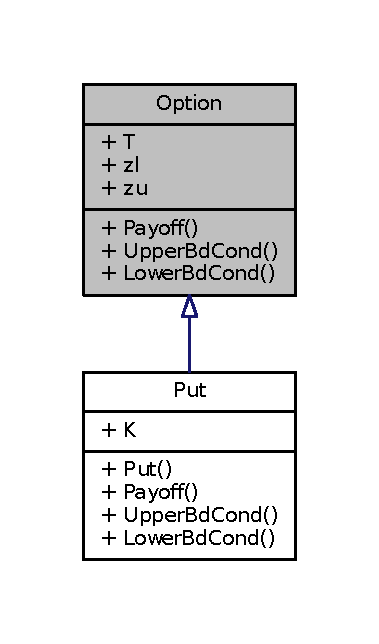
\includegraphics[width=182pt]{classOption__inherit__graph}
\end{center}
\end{figure}


Collaboration diagram for Option\+:\nopagebreak
\begin{figure}[H]
\begin{center}
\leavevmode
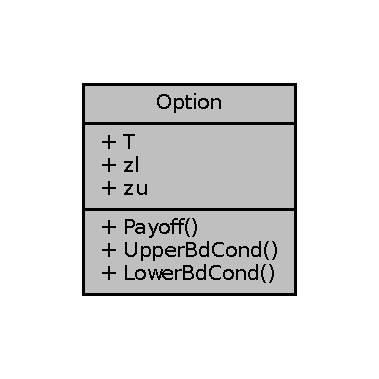
\includegraphics[width=182pt]{classOption__coll__graph}
\end{center}
\end{figure}
\subsection*{Public Member Functions}
\begin{DoxyCompactItemize}
\item 
virtual double \hyperlink{classOption_a10f2917f21055a1beb890353e53e0865}{Payoff} (double z)=0
\item 
virtual double \hyperlink{classOption_a8f27761a53a9f0e7746b9358405a03f7}{Upper\+Bd\+Cond} (\hyperlink{classBSModel}{B\+S\+Model} $\ast$Ptr\+Model, double t)=0
\item 
virtual double \hyperlink{classOption_afda338619f5646c0cb9e6cd5c83717f9}{Lower\+Bd\+Cond} (\hyperlink{classBSModel}{B\+S\+Model} $\ast$Ptr\+Model, double t)=0
\end{DoxyCompactItemize}
\subsection*{Public Attributes}
\begin{DoxyCompactItemize}
\item 
double \hyperlink{classOption_ae583dd6d430a3b428014efa942605d54}{T}
\item 
double \hyperlink{classOption_a37c65100e75876d4f4b76e8647c6702d}{zl}
\item 
double \hyperlink{classOption_aa80c6f304df39def3df2bf26afbbfe79}{zu}
\end{DoxyCompactItemize}


\subsection{Detailed Description}


Definition at line \hyperlink{Options_8h_source_l00023}{23} of file \hyperlink{Options_8h_source}{Options.\+h}.



\subsection{Member Function Documentation}
\hypertarget{classOption_afda338619f5646c0cb9e6cd5c83717f9}{\index{Option@{Option}!Lower\+Bd\+Cond@{Lower\+Bd\+Cond}}
\index{Lower\+Bd\+Cond@{Lower\+Bd\+Cond}!Option@{Option}}
\subsubsection[{Lower\+Bd\+Cond}]{\setlength{\rightskip}{0pt plus 5cm}virtual double Option\+::\+Lower\+Bd\+Cond (
\begin{DoxyParamCaption}
\item[{{\bf B\+S\+Model} $\ast$}]{Ptr\+Model, }
\item[{double}]{t}
\end{DoxyParamCaption}
)\hspace{0.3cm}{\ttfamily [pure virtual]}}}\label{classOption_afda338619f5646c0cb9e6cd5c83717f9}


Implemented in \hyperlink{classPut_ab07d0f1d939f267861484f645d71c9c5}{Put}.



Here is the caller graph for this function\+:\nopagebreak
\begin{figure}[H]
\begin{center}
\leavevmode
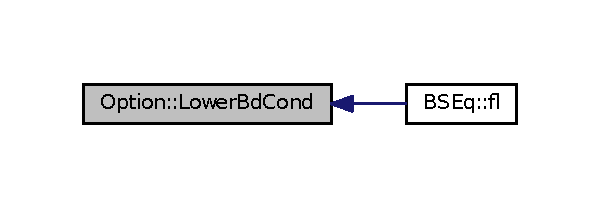
\includegraphics[width=288pt]{classOption_afda338619f5646c0cb9e6cd5c83717f9_icgraph}
\end{center}
\end{figure}


\hypertarget{classOption_a10f2917f21055a1beb890353e53e0865}{\index{Option@{Option}!Payoff@{Payoff}}
\index{Payoff@{Payoff}!Option@{Option}}
\subsubsection[{Payoff}]{\setlength{\rightskip}{0pt plus 5cm}virtual double Option\+::\+Payoff (
\begin{DoxyParamCaption}
\item[{double}]{z}
\end{DoxyParamCaption}
)\hspace{0.3cm}{\ttfamily [pure virtual]}}}\label{classOption_a10f2917f21055a1beb890353e53e0865}


Implemented in \hyperlink{classPut_ae2bbadeb2c9f05644ef9b9af97ad7520}{Put}.



Here is the caller graph for this function\+:\nopagebreak
\begin{figure}[H]
\begin{center}
\leavevmode
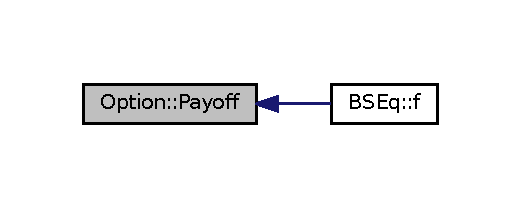
\includegraphics[width=250pt]{classOption_a10f2917f21055a1beb890353e53e0865_icgraph}
\end{center}
\end{figure}


\hypertarget{classOption_a8f27761a53a9f0e7746b9358405a03f7}{\index{Option@{Option}!Upper\+Bd\+Cond@{Upper\+Bd\+Cond}}
\index{Upper\+Bd\+Cond@{Upper\+Bd\+Cond}!Option@{Option}}
\subsubsection[{Upper\+Bd\+Cond}]{\setlength{\rightskip}{0pt plus 5cm}virtual double Option\+::\+Upper\+Bd\+Cond (
\begin{DoxyParamCaption}
\item[{{\bf B\+S\+Model} $\ast$}]{Ptr\+Model, }
\item[{double}]{t}
\end{DoxyParamCaption}
)\hspace{0.3cm}{\ttfamily [pure virtual]}}}\label{classOption_a8f27761a53a9f0e7746b9358405a03f7}


Implemented in \hyperlink{classPut_ac15aea264781b4f426b68918ab73a27d}{Put}.



Here is the caller graph for this function\+:\nopagebreak
\begin{figure}[H]
\begin{center}
\leavevmode
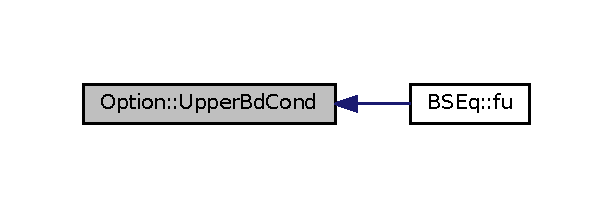
\includegraphics[width=294pt]{classOption_a8f27761a53a9f0e7746b9358405a03f7_icgraph}
\end{center}
\end{figure}




\subsection{Member Data Documentation}
\hypertarget{classOption_ae583dd6d430a3b428014efa942605d54}{\index{Option@{Option}!T@{T}}
\index{T@{T}!Option@{Option}}
\subsubsection[{T}]{\setlength{\rightskip}{0pt plus 5cm}double Option\+::\+T}}\label{classOption_ae583dd6d430a3b428014efa942605d54}


Definition at line \hyperlink{Options_8h_source_l00025}{25} of file \hyperlink{Options_8h_source}{Options.\+h}.

\hypertarget{classOption_a37c65100e75876d4f4b76e8647c6702d}{\index{Option@{Option}!zl@{zl}}
\index{zl@{zl}!Option@{Option}}
\subsubsection[{zl}]{\setlength{\rightskip}{0pt plus 5cm}double Option\+::zl}}\label{classOption_a37c65100e75876d4f4b76e8647c6702d}


Definition at line \hyperlink{Options_8h_source_l00026}{26} of file \hyperlink{Options_8h_source}{Options.\+h}.

\hypertarget{classOption_aa80c6f304df39def3df2bf26afbbfe79}{\index{Option@{Option}!zu@{zu}}
\index{zu@{zu}!Option@{Option}}
\subsubsection[{zu}]{\setlength{\rightskip}{0pt plus 5cm}double Option\+::zu}}\label{classOption_aa80c6f304df39def3df2bf26afbbfe79}


Definition at line \hyperlink{Options_8h_source_l00027}{27} of file \hyperlink{Options_8h_source}{Options.\+h}.



The documentation for this class was generated from the following file\+:\begin{DoxyCompactItemize}
\item 
\hyperlink{Options_8h}{Options.\+h}\end{DoxyCompactItemize}

\hypertarget{classParabPDE}{\section{Parab\+P\+D\+E Class Reference}
\label{classParabPDE}\index{Parab\+P\+D\+E@{Parab\+P\+D\+E}}
}


{\ttfamily \#include $<$Parab\+P\+D\+E.\+h$>$}



Inheritance diagram for Parab\+P\+D\+E\+:\nopagebreak
\begin{figure}[H]
\begin{center}
\leavevmode
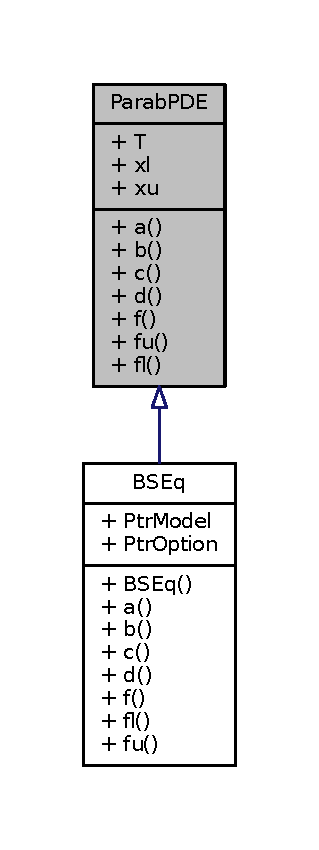
\includegraphics[width=153pt]{classParabPDE__inherit__graph}
\end{center}
\end{figure}


Collaboration diagram for Parab\+P\+D\+E\+:\nopagebreak
\begin{figure}[H]
\begin{center}
\leavevmode
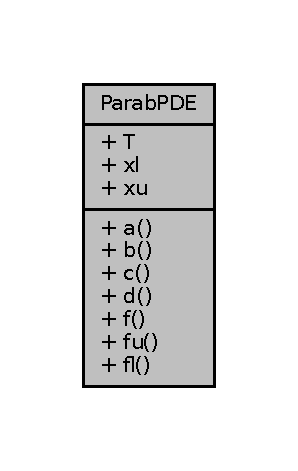
\includegraphics[width=143pt]{classParabPDE__coll__graph}
\end{center}
\end{figure}
\subsection*{Public Member Functions}
\begin{DoxyCompactItemize}
\item 
virtual double \hyperlink{classParabPDE_a809e251d53ff62714bc8a30e45cc88a5}{a} (double t, double x)=0
\item 
virtual double \hyperlink{classParabPDE_ab98c81bf66471fa6f67dc17b9123bda6}{b} (double t, double x)=0
\item 
virtual double \hyperlink{classParabPDE_aebec9339309e456136ecd0c3b4a74bb0}{c} (double t, double x)=0
\item 
virtual double \hyperlink{classParabPDE_a13531e677a97660f56f88fc8a9f2c593}{d} (double t, double x)=0
\item 
virtual double \hyperlink{classParabPDE_a099b6ba266fb033de9901a60dc935ddf}{f} (double x)=0
\item 
virtual double \hyperlink{classParabPDE_a8a1850597550bf8aab3b5dca2aed6ff8}{fu} (double t)=0
\item 
virtual double \hyperlink{classParabPDE_aa083d2745f44daba57ad296749eb7ec0}{fl} (double t)=0
\end{DoxyCompactItemize}
\subsection*{Public Attributes}
\begin{DoxyCompactItemize}
\item 
double \hyperlink{classParabPDE_accce3d4cc39e47137915a47b4edd838e}{T}
\item 
double \hyperlink{classParabPDE_aa75c941c87400c92781c74e1e4f5ae5e}{xl}
\item 
double \hyperlink{classParabPDE_a5e4f6911cba231072c0ed4b6b4462b8a}{xu}
\end{DoxyCompactItemize}


\subsection{Detailed Description}


Definition at line \hyperlink{ParabPDE_8h_source_l00034}{34} of file \hyperlink{ParabPDE_8h_source}{Parab\+P\+D\+E.\+h}.



\subsection{Member Function Documentation}
\hypertarget{classParabPDE_a809e251d53ff62714bc8a30e45cc88a5}{\index{Parab\+P\+D\+E@{Parab\+P\+D\+E}!a@{a}}
\index{a@{a}!Parab\+P\+D\+E@{Parab\+P\+D\+E}}
\subsubsection[{a}]{\setlength{\rightskip}{0pt plus 5cm}virtual double Parab\+P\+D\+E\+::a (
\begin{DoxyParamCaption}
\item[{double}]{t, }
\item[{double}]{x}
\end{DoxyParamCaption}
)\hspace{0.3cm}{\ttfamily [pure virtual]}}}\label{classParabPDE_a809e251d53ff62714bc8a30e45cc88a5}


Implemented in \hyperlink{classBSEq_aac9b72618a86b764022bc2f8a0623b0c}{B\+S\+Eq}.



Here is the caller graph for this function\+:\nopagebreak
\begin{figure}[H]
\begin{center}
\leavevmode
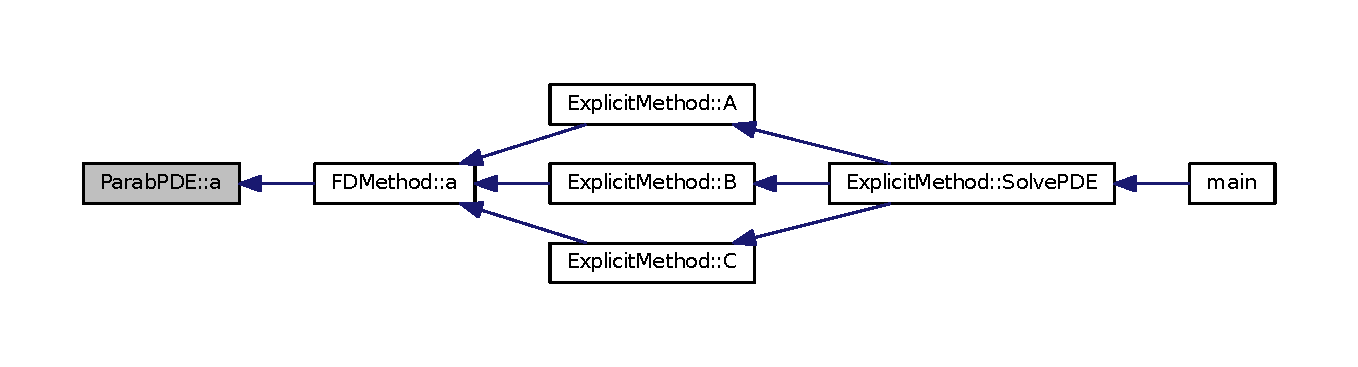
\includegraphics[width=350pt]{classParabPDE_a809e251d53ff62714bc8a30e45cc88a5_icgraph}
\end{center}
\end{figure}


\hypertarget{classParabPDE_ab98c81bf66471fa6f67dc17b9123bda6}{\index{Parab\+P\+D\+E@{Parab\+P\+D\+E}!b@{b}}
\index{b@{b}!Parab\+P\+D\+E@{Parab\+P\+D\+E}}
\subsubsection[{b}]{\setlength{\rightskip}{0pt plus 5cm}virtual double Parab\+P\+D\+E\+::b (
\begin{DoxyParamCaption}
\item[{double}]{t, }
\item[{double}]{x}
\end{DoxyParamCaption}
)\hspace{0.3cm}{\ttfamily [pure virtual]}}}\label{classParabPDE_ab98c81bf66471fa6f67dc17b9123bda6}


Implemented in \hyperlink{classBSEq_a7b0a00c216ae383f5a768c8efd42e672}{B\+S\+Eq}.



Here is the caller graph for this function\+:\nopagebreak
\begin{figure}[H]
\begin{center}
\leavevmode
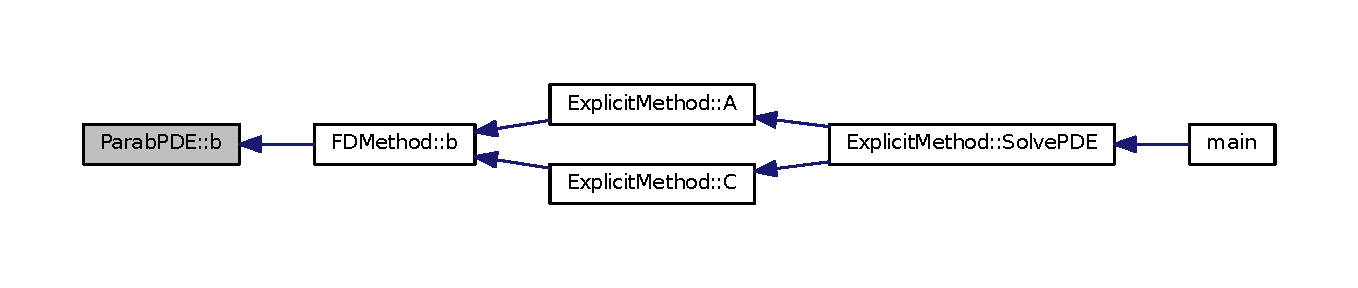
\includegraphics[width=350pt]{classParabPDE_ab98c81bf66471fa6f67dc17b9123bda6_icgraph}
\end{center}
\end{figure}


\hypertarget{classParabPDE_aebec9339309e456136ecd0c3b4a74bb0}{\index{Parab\+P\+D\+E@{Parab\+P\+D\+E}!c@{c}}
\index{c@{c}!Parab\+P\+D\+E@{Parab\+P\+D\+E}}
\subsubsection[{c}]{\setlength{\rightskip}{0pt plus 5cm}virtual double Parab\+P\+D\+E\+::c (
\begin{DoxyParamCaption}
\item[{double}]{t, }
\item[{double}]{x}
\end{DoxyParamCaption}
)\hspace{0.3cm}{\ttfamily [pure virtual]}}}\label{classParabPDE_aebec9339309e456136ecd0c3b4a74bb0}


Implemented in \hyperlink{classBSEq_aa63fc29fedf4ef53ace9499fab4d7aba}{B\+S\+Eq}.



Here is the caller graph for this function\+:\nopagebreak
\begin{figure}[H]
\begin{center}
\leavevmode
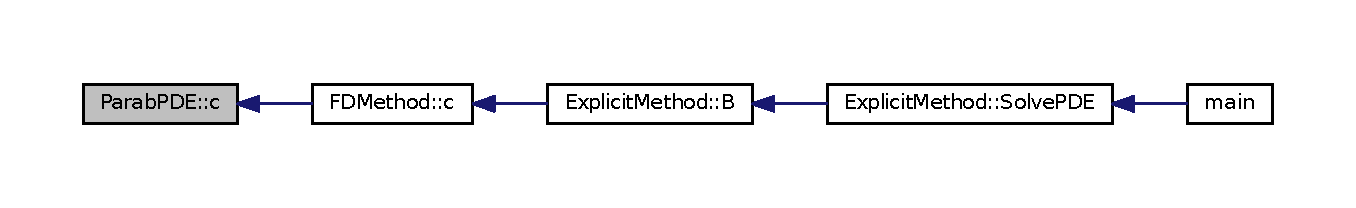
\includegraphics[width=350pt]{classParabPDE_aebec9339309e456136ecd0c3b4a74bb0_icgraph}
\end{center}
\end{figure}


\hypertarget{classParabPDE_a13531e677a97660f56f88fc8a9f2c593}{\index{Parab\+P\+D\+E@{Parab\+P\+D\+E}!d@{d}}
\index{d@{d}!Parab\+P\+D\+E@{Parab\+P\+D\+E}}
\subsubsection[{d}]{\setlength{\rightskip}{0pt plus 5cm}virtual double Parab\+P\+D\+E\+::d (
\begin{DoxyParamCaption}
\item[{double}]{t, }
\item[{double}]{x}
\end{DoxyParamCaption}
)\hspace{0.3cm}{\ttfamily [pure virtual]}}}\label{classParabPDE_a13531e677a97660f56f88fc8a9f2c593}


Implemented in \hyperlink{classBSEq_ae01526739bc51e813dfdb880585aefc0}{B\+S\+Eq}.



Here is the caller graph for this function\+:\nopagebreak
\begin{figure}[H]
\begin{center}
\leavevmode
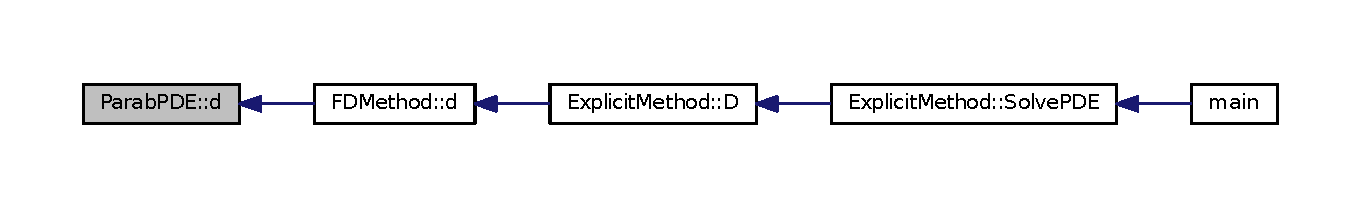
\includegraphics[width=350pt]{classParabPDE_a13531e677a97660f56f88fc8a9f2c593_icgraph}
\end{center}
\end{figure}


\hypertarget{classParabPDE_a099b6ba266fb033de9901a60dc935ddf}{\index{Parab\+P\+D\+E@{Parab\+P\+D\+E}!f@{f}}
\index{f@{f}!Parab\+P\+D\+E@{Parab\+P\+D\+E}}
\subsubsection[{f}]{\setlength{\rightskip}{0pt plus 5cm}virtual double Parab\+P\+D\+E\+::f (
\begin{DoxyParamCaption}
\item[{double}]{x}
\end{DoxyParamCaption}
)\hspace{0.3cm}{\ttfamily [pure virtual]}}}\label{classParabPDE_a099b6ba266fb033de9901a60dc935ddf}


Implemented in \hyperlink{classBSEq_a6c81cef2ec102bc86bc8ff6378a2a519}{B\+S\+Eq}.



Here is the caller graph for this function\+:\nopagebreak
\begin{figure}[H]
\begin{center}
\leavevmode
\includegraphics[width=350pt]{classParabPDE_a099b6ba266fb033de9901a60dc935ddf_icgraph}
\end{center}
\end{figure}


\hypertarget{classParabPDE_aa083d2745f44daba57ad296749eb7ec0}{\index{Parab\+P\+D\+E@{Parab\+P\+D\+E}!fl@{fl}}
\index{fl@{fl}!Parab\+P\+D\+E@{Parab\+P\+D\+E}}
\subsubsection[{fl}]{\setlength{\rightskip}{0pt plus 5cm}virtual double Parab\+P\+D\+E\+::fl (
\begin{DoxyParamCaption}
\item[{double}]{t}
\end{DoxyParamCaption}
)\hspace{0.3cm}{\ttfamily [pure virtual]}}}\label{classParabPDE_aa083d2745f44daba57ad296749eb7ec0}


Implemented in \hyperlink{classBSEq_a5bde9ad3db5d94df77c78929de7f2717}{B\+S\+Eq}.



Here is the caller graph for this function\+:\nopagebreak
\begin{figure}[H]
\begin{center}
\leavevmode
\includegraphics[width=350pt]{classParabPDE_aa083d2745f44daba57ad296749eb7ec0_icgraph}
\end{center}
\end{figure}


\hypertarget{classParabPDE_a8a1850597550bf8aab3b5dca2aed6ff8}{\index{Parab\+P\+D\+E@{Parab\+P\+D\+E}!fu@{fu}}
\index{fu@{fu}!Parab\+P\+D\+E@{Parab\+P\+D\+E}}
\subsubsection[{fu}]{\setlength{\rightskip}{0pt plus 5cm}virtual double Parab\+P\+D\+E\+::fu (
\begin{DoxyParamCaption}
\item[{double}]{t}
\end{DoxyParamCaption}
)\hspace{0.3cm}{\ttfamily [pure virtual]}}}\label{classParabPDE_a8a1850597550bf8aab3b5dca2aed6ff8}


Implemented in \hyperlink{classBSEq_acebc22c41d04659861ef346d988de565}{B\+S\+Eq}.



Here is the caller graph for this function\+:\nopagebreak
\begin{figure}[H]
\begin{center}
\leavevmode
\includegraphics[width=350pt]{classParabPDE_a8a1850597550bf8aab3b5dca2aed6ff8_icgraph}
\end{center}
\end{figure}




\subsection{Member Data Documentation}
\hypertarget{classParabPDE_accce3d4cc39e47137915a47b4edd838e}{\index{Parab\+P\+D\+E@{Parab\+P\+D\+E}!T@{T}}
\index{T@{T}!Parab\+P\+D\+E@{Parab\+P\+D\+E}}
\subsubsection[{T}]{\setlength{\rightskip}{0pt plus 5cm}double Parab\+P\+D\+E\+::\+T}}\label{classParabPDE_accce3d4cc39e47137915a47b4edd838e}


Definition at line \hyperlink{ParabPDE_8h_source_l00037}{37} of file \hyperlink{ParabPDE_8h_source}{Parab\+P\+D\+E.\+h}.

\hypertarget{classParabPDE_aa75c941c87400c92781c74e1e4f5ae5e}{\index{Parab\+P\+D\+E@{Parab\+P\+D\+E}!xl@{xl}}
\index{xl@{xl}!Parab\+P\+D\+E@{Parab\+P\+D\+E}}
\subsubsection[{xl}]{\setlength{\rightskip}{0pt plus 5cm}double Parab\+P\+D\+E\+::xl}}\label{classParabPDE_aa75c941c87400c92781c74e1e4f5ae5e}


Definition at line \hyperlink{ParabPDE_8h_source_l00038}{38} of file \hyperlink{ParabPDE_8h_source}{Parab\+P\+D\+E.\+h}.

\hypertarget{classParabPDE_a5e4f6911cba231072c0ed4b6b4462b8a}{\index{Parab\+P\+D\+E@{Parab\+P\+D\+E}!xu@{xu}}
\index{xu@{xu}!Parab\+P\+D\+E@{Parab\+P\+D\+E}}
\subsubsection[{xu}]{\setlength{\rightskip}{0pt plus 5cm}double Parab\+P\+D\+E\+::xu}}\label{classParabPDE_a5e4f6911cba231072c0ed4b6b4462b8a}


Definition at line \hyperlink{ParabPDE_8h_source_l00039}{39} of file \hyperlink{ParabPDE_8h_source}{Parab\+P\+D\+E.\+h}.



The documentation for this class was generated from the following file\+:\begin{DoxyCompactItemize}
\item 
\hyperlink{ParabPDE_8h}{Parab\+P\+D\+E.\+h}\end{DoxyCompactItemize}

\hypertarget{classPut}{\section{Put Class Reference}
\label{classPut}\index{Put@{Put}}
}


{\ttfamily \#include $<$Options.\+h$>$}



Inheritance diagram for Put\+:\nopagebreak
\begin{figure}[H]
\begin{center}
\leavevmode
\includegraphics[width=182pt]{classPut__inherit__graph}
\end{center}
\end{figure}


Collaboration diagram for Put\+:\nopagebreak
\begin{figure}[H]
\begin{center}
\leavevmode
\includegraphics[width=182pt]{classPut__coll__graph}
\end{center}
\end{figure}
\subsection*{Public Member Functions}
\begin{DoxyCompactItemize}
\item 
\hyperlink{classPut_a8a846b5650bb0d677c251a114c8d32e0}{Put} (double K\+\_\+, double T\+\_\+, double zl\+\_\+, double zu\+\_\+)
\item 
double \hyperlink{classPut_ae2bbadeb2c9f05644ef9b9af97ad7520}{Payoff} (double z)
\item 
double \hyperlink{classPut_ac15aea264781b4f426b68918ab73a27d}{Upper\+Bd\+Cond} (\hyperlink{classBSModel}{B\+S\+Model} $\ast$Ptr\+Model, double t)
\item 
double \hyperlink{classPut_ab07d0f1d939f267861484f645d71c9c5}{Lower\+Bd\+Cond} (\hyperlink{classBSModel}{B\+S\+Model} $\ast$Ptr\+Model, double t)
\end{DoxyCompactItemize}
\subsection*{Public Attributes}
\begin{DoxyCompactItemize}
\item 
double \hyperlink{classPut_aa8d5c1c7465fd311ddaf33533038f959}{K}
\end{DoxyCompactItemize}


\subsection{Detailed Description}


Definition at line \hyperlink{Options_8h_source_l00034}{34} of file \hyperlink{Options_8h_source}{Options.\+h}.



\subsection{Constructor \& Destructor Documentation}
\hypertarget{classPut_a8a846b5650bb0d677c251a114c8d32e0}{\index{Put@{Put}!Put@{Put}}
\index{Put@{Put}!Put@{Put}}
\subsubsection[{Put}]{\setlength{\rightskip}{0pt plus 5cm}Put\+::\+Put (
\begin{DoxyParamCaption}
\item[{double}]{K\+\_\+, }
\item[{double}]{T\+\_\+, }
\item[{double}]{zl\+\_\+, }
\item[{double}]{zu\+\_\+}
\end{DoxyParamCaption}
)\hspace{0.3cm}{\ttfamily [inline]}}}\label{classPut_a8a846b5650bb0d677c251a114c8d32e0}


Definition at line \hyperlink{Options_8h_source_l00038}{38} of file \hyperlink{Options_8h_source}{Options.\+h}.



\subsection{Member Function Documentation}
\hypertarget{classPut_ab07d0f1d939f267861484f645d71c9c5}{\index{Put@{Put}!Lower\+Bd\+Cond@{Lower\+Bd\+Cond}}
\index{Lower\+Bd\+Cond@{Lower\+Bd\+Cond}!Put@{Put}}
\subsubsection[{Lower\+Bd\+Cond}]{\setlength{\rightskip}{0pt plus 5cm}double Put\+::\+Lower\+Bd\+Cond (
\begin{DoxyParamCaption}
\item[{{\bf B\+S\+Model} $\ast$}]{Ptr\+Model, }
\item[{double}]{t}
\end{DoxyParamCaption}
)\hspace{0.3cm}{\ttfamily [virtual]}}}\label{classPut_ab07d0f1d939f267861484f645d71c9c5}


Implements \hyperlink{classOption_afda338619f5646c0cb9e6cd5c83717f9}{Option}.



Definition at line \hyperlink{Options_8cpp_source_l00035}{35} of file \hyperlink{Options_8cpp_source}{Options.\+cpp}.

\hypertarget{classPut_ae2bbadeb2c9f05644ef9b9af97ad7520}{\index{Put@{Put}!Payoff@{Payoff}}
\index{Payoff@{Payoff}!Put@{Put}}
\subsubsection[{Payoff}]{\setlength{\rightskip}{0pt plus 5cm}double Put\+::\+Payoff (
\begin{DoxyParamCaption}
\item[{double}]{z}
\end{DoxyParamCaption}
)\hspace{0.3cm}{\ttfamily [virtual]}}}\label{classPut_ae2bbadeb2c9f05644ef9b9af97ad7520}


Implements \hyperlink{classOption_a10f2917f21055a1beb890353e53e0865}{Option}.



Definition at line \hyperlink{Options_8cpp_source_l00022}{22} of file \hyperlink{Options_8cpp_source}{Options.\+cpp}.

\hypertarget{classPut_ac15aea264781b4f426b68918ab73a27d}{\index{Put@{Put}!Upper\+Bd\+Cond@{Upper\+Bd\+Cond}}
\index{Upper\+Bd\+Cond@{Upper\+Bd\+Cond}!Put@{Put}}
\subsubsection[{Upper\+Bd\+Cond}]{\setlength{\rightskip}{0pt plus 5cm}double Put\+::\+Upper\+Bd\+Cond (
\begin{DoxyParamCaption}
\item[{{\bf B\+S\+Model} $\ast$}]{Ptr\+Model, }
\item[{double}]{t}
\end{DoxyParamCaption}
)\hspace{0.3cm}{\ttfamily [virtual]}}}\label{classPut_ac15aea264781b4f426b68918ab73a27d}


Implements \hyperlink{classOption_a8f27761a53a9f0e7746b9358405a03f7}{Option}.



Definition at line \hyperlink{Options_8cpp_source_l00030}{30} of file \hyperlink{Options_8cpp_source}{Options.\+cpp}.



\subsection{Member Data Documentation}
\hypertarget{classPut_aa8d5c1c7465fd311ddaf33533038f959}{\index{Put@{Put}!K@{K}}
\index{K@{K}!Put@{Put}}
\subsubsection[{K}]{\setlength{\rightskip}{0pt plus 5cm}double Put\+::\+K}}\label{classPut_aa8d5c1c7465fd311ddaf33533038f959}


Definition at line \hyperlink{Options_8h_source_l00036}{36} of file \hyperlink{Options_8h_source}{Options.\+h}.



The documentation for this class was generated from the following files\+:\begin{DoxyCompactItemize}
\item 
\hyperlink{Options_8h}{Options.\+h}\item 
\hyperlink{Options_8cpp}{Options.\+cpp}\end{DoxyCompactItemize}

\chapter{File Documentation}
\hypertarget{BSEq_8cpp}{\section{B\+S\+Eq.\+cpp File Reference}
\label{BSEq_8cpp}\index{B\+S\+Eq.\+cpp@{B\+S\+Eq.\+cpp}}
}


implements a class representing the Black--Scholes equation.  


{\ttfamily \#include $<$cmath$>$}\\*
{\ttfamily \#include \char`\"{}B\+S\+Eq.\+h\char`\"{}}\\*
Include dependency graph for B\+S\+Eq.\+cpp\+:\nopagebreak
\begin{figure}[H]
\begin{center}
\leavevmode
\includegraphics[width=319pt]{BSEq_8cpp__incl}
\end{center}
\end{figure}


\subsection{Detailed Description}
A typical reason for studying parabolic partial differential equations in finance is the Black–-\/\+Scholes equation.

Let $ S(t) $ denote the price at time $ t $ of the underlying asset under the Black–-\/\+Scholes equation. Suppose that at time $ t $ the price of a financial derivative $ H(t) $ can be expressed using a function $ u $, defined as\+: \[ H(t) = u(t, S (t)). \] If $ u $ is a $ C^{1,2} $ function on $ [0,T)\times \mathbb{R} $, then the Black--Scholes equation can be used to solve for $ u $.

When $ u(t, S(t)) $ is the value of an option with expiry date $ T $ and payoff $ H(T) = h(S(T)) $, then $ u(T, S(T)) = h(S(T)) $, hence the terminal condition is \[ u(T, z) = h(z). \] The lower and upper boundary conditions depend on the type of the option we wish to price. They can usually be derived from heuristic or arbitrage arguments.

For example, for a {\bfseries put option} with expiry date $ T $ and strike price $ K $, if $ S(t) $ is high, then the option is practically worthless since it is unlikely to be exercised. This means that we can consider a sufficiently large $ z_u $ and set\+: \[ u(t, zu) = h^{put}_u(t) = 0. \] Also, if $ S(t) $ is close to zero, then we can assume that we are almost certain to exercise the put at expiry and obtain a payoff close to $ K $. Considering a sufficiently small positive $ z_l $ we can therefore set\+: \[ u(t, zl) = h^{put}_l(t) = exp(-r(T - t))K. \]

\begin{DoxyWarning}{Warning}
This code is also listed and fully explained in the book $\ast$$\ast$\+Numerical Methods in Finance with C++$\ast$$\ast$ by Maciej Capiński and Tomasz Zastawniak, published in September 2012.
\end{DoxyWarning}
\begin{DoxyAuthor}{Author}
\+: Eduardo J. Sanchez (ejspeiro) -\/ ejspeiro at gmail dot com 
\end{DoxyAuthor}


Definition in file \hyperlink{BSEq_8cpp_source}{B\+S\+Eq.\+cpp}.


\hypertarget{BSEq_8cpp_source}{\section{B\+S\+Eq.\+cpp}
}

\begin{DoxyCode}
00001 
00050 \textcolor{preprocessor}{#include <cmath>}
00051 
00052 \textcolor{preprocessor}{#include "\hyperlink{BSEq_8h}{BSEq.h}"}
00053 
\hypertarget{BSEq_8cpp_source_l00054}{}\hyperlink{classBSEq_a3545b5fe078c573514666f07e3d516b2}{00054} \hyperlink{classBSEq_a3545b5fe078c573514666f07e3d516b2}{BSEq::BSEq}(\hyperlink{classBSModel}{BSModel}* PtrModel\_, \hyperlink{classOption}{Option}* PtrOption\_) \{
00055 
00056   \hyperlink{classBSEq_a44b63f8349d8ab91a1fb8fc026cdf142}{PtrModel} = PtrModel\_;
00057   \hyperlink{classBSEq_a280b15d8a4cd19d1aefc9feeb35a75bb}{PtrOption} = PtrOption\_;
00058   \hyperlink{classParabPDE_accce3d4cc39e47137915a47b4edd838e}{T} = \hyperlink{classBSEq_a280b15d8a4cd19d1aefc9feeb35a75bb}{PtrOption}->\hyperlink{classOption_ae583dd6d430a3b428014efa942605d54}{T};
00059   \hyperlink{classParabPDE_aa75c941c87400c92781c74e1e4f5ae5e}{xl} = \hyperlink{classBSEq_a280b15d8a4cd19d1aefc9feeb35a75bb}{PtrOption}->\hyperlink{classOption_a37c65100e75876d4f4b76e8647c6702d}{zl};
00060   \hyperlink{classParabPDE_a5e4f6911cba231072c0ed4b6b4462b8a}{xu} = \hyperlink{classBSEq_a280b15d8a4cd19d1aefc9feeb35a75bb}{PtrOption}->\hyperlink{classOption_aa80c6f304df39def3df2bf26afbbfe79}{zu};
00061 \}
00062 
\hypertarget{BSEq_8cpp_source_l00063}{}\hyperlink{classBSEq_aac9b72618a86b764022bc2f8a0623b0c}{00063} \textcolor{keywordtype}{double} \hyperlink{classBSEq_aac9b72618a86b764022bc2f8a0623b0c}{BSEq::a}(\textcolor{keywordtype}{double} t, \textcolor{keywordtype}{double} z) \{
00064 
00065   \textcolor{keywordflow}{return} -0.5*pow(\hyperlink{classBSEq_a44b63f8349d8ab91a1fb8fc026cdf142}{PtrModel}->\hyperlink{classBSModel_a1267641043c16cd9baf2eb242320f0d3}{sigma}*z, 2.0);
00066 \}
00067 
\hypertarget{BSEq_8cpp_source_l00068}{}\hyperlink{classBSEq_a7b0a00c216ae383f5a768c8efd42e672}{00068} \textcolor{keywordtype}{double} \hyperlink{classBSEq_a7b0a00c216ae383f5a768c8efd42e672}{BSEq::b}(\textcolor{keywordtype}{double} t, \textcolor{keywordtype}{double} z) \{
00069 
00070   \textcolor{keywordflow}{return} -\hyperlink{classBSEq_a44b63f8349d8ab91a1fb8fc026cdf142}{PtrModel}->\hyperlink{classBSModel_add3230c0df8e47623116b439598c0de3}{r}*z;
00071 \}
00072 
\hypertarget{BSEq_8cpp_source_l00073}{}\hyperlink{classBSEq_aa63fc29fedf4ef53ace9499fab4d7aba}{00073} \textcolor{keywordtype}{double} \hyperlink{classBSEq_aa63fc29fedf4ef53ace9499fab4d7aba}{BSEq::c}(\textcolor{keywordtype}{double} t, \textcolor{keywordtype}{double} z) \{
00074 
00075   \textcolor{keywordflow}{return} \hyperlink{classBSEq_a44b63f8349d8ab91a1fb8fc026cdf142}{PtrModel}->\hyperlink{classBSModel_add3230c0df8e47623116b439598c0de3}{r};
00076 \}
00077 
\hypertarget{BSEq_8cpp_source_l00078}{}\hyperlink{classBSEq_ae01526739bc51e813dfdb880585aefc0}{00078} \textcolor{keywordtype}{double} \hyperlink{classBSEq_ae01526739bc51e813dfdb880585aefc0}{BSEq::d}(\textcolor{keywordtype}{double} t, \textcolor{keywordtype}{double} z) \{
00079 
00080   \textcolor{keywordflow}{return} 0.0;
00081 \}
00082 
\hypertarget{BSEq_8cpp_source_l00083}{}\hyperlink{classBSEq_a6c81cef2ec102bc86bc8ff6378a2a519}{00083} \textcolor{keywordtype}{double} \hyperlink{classBSEq_a6c81cef2ec102bc86bc8ff6378a2a519}{BSEq::f}(\textcolor{keywordtype}{double} z) \{
00084 
00085   \textcolor{keywordflow}{return} \hyperlink{classBSEq_a280b15d8a4cd19d1aefc9feeb35a75bb}{PtrOption}->\hyperlink{classOption_a10f2917f21055a1beb890353e53e0865}{Payoff}(z);
00086 \}
00087 
\hypertarget{BSEq_8cpp_source_l00088}{}\hyperlink{classBSEq_a5bde9ad3db5d94df77c78929de7f2717}{00088} \textcolor{keywordtype}{double} \hyperlink{classBSEq_a5bde9ad3db5d94df77c78929de7f2717}{BSEq::fl}(\textcolor{keywordtype}{double} t) \{
00089 
00090   \textcolor{keywordflow}{return} \hyperlink{classBSEq_a280b15d8a4cd19d1aefc9feeb35a75bb}{PtrOption}->\hyperlink{classOption_afda338619f5646c0cb9e6cd5c83717f9}{LowerBdCond}(\hyperlink{classBSEq_a44b63f8349d8ab91a1fb8fc026cdf142}{PtrModel}, t);
00091 \}
00092 
\hypertarget{BSEq_8cpp_source_l00093}{}\hyperlink{classBSEq_acebc22c41d04659861ef346d988de565}{00093} \textcolor{keywordtype}{double} \hyperlink{classBSEq_acebc22c41d04659861ef346d988de565}{BSEq::fu}(\textcolor{keywordtype}{double} t) \{
00094 
00095   \textcolor{keywordflow}{return} \hyperlink{classBSEq_a280b15d8a4cd19d1aefc9feeb35a75bb}{PtrOption}->\hyperlink{classOption_a8f27761a53a9f0e7746b9358405a03f7}{UpperBdCond}(\hyperlink{classBSEq_a44b63f8349d8ab91a1fb8fc026cdf142}{PtrModel}, t);
00096 \}
\end{DoxyCode}

\hypertarget{BSEq_8h}{\section{B\+S\+Eq.\+h File Reference}
\label{BSEq_8h}\index{B\+S\+Eq.\+h@{B\+S\+Eq.\+h}}
}


Defines a class representing the Black--Scholes equation.  


{\ttfamily \#include \char`\"{}B\+S\+Model01.\+h\char`\"{}}\\*
{\ttfamily \#include \char`\"{}Options.\+h\char`\"{}}\\*
{\ttfamily \#include \char`\"{}Parab\+P\+D\+E.\+h\char`\"{}}\\*
Include dependency graph for B\+S\+Eq.\+h\+:\nopagebreak
\begin{figure}[H]
\begin{center}
\leavevmode
\includegraphics[width=319pt]{BSEq_8h__incl}
\end{center}
\end{figure}
This graph shows which files directly or indirectly include this file\+:\nopagebreak
\begin{figure}[H]
\begin{center}
\leavevmode
\includegraphics[width=232pt]{BSEq_8h__dep__incl}
\end{center}
\end{figure}
\subsection*{Classes}
\begin{DoxyCompactItemize}
\item 
class \hyperlink{classBSEq}{B\+S\+Eq}
\end{DoxyCompactItemize}


\subsection{Detailed Description}
A typical reason for studying parabolic partial differential equations in finance is the Black–-\/\+Scholes equation.

Let $ S(t) $ denote the price at time $ t $ of the underlying asset under the Black–-\/\+Scholes equation. Suppose that at time $ t $ the price of a financial derivative $ H(t) $ can be expressed using a function $ u $, defined as\+: \[ H(t) = u(t, S (t)). \] If $ u $ is a $ C^{1,2} $ function on $ [0,T)\times \mathbb{R} $, then the Black--Scholes equation can be used to solve for $ u $.

When $ u(t, S(t)) $ is the value of an option with expiry date $ T $ and payoff $ H(T) = h(S(T)) $, then $ u(T, S(T)) = h(S(T)) $, hence the terminal condition is \[ u(T, z) = h(z). \] The lower and upper boundary conditions depend on the type of the option we wish to price. They can usually be derived from heuristic or arbitrage arguments.

For example, for a {\bfseries put option} with expiry date $ T $ and strike price $ K $, if $ S(t) $ is high, then the option is practically worthless since it is unlikely to be exercised. This means that we can consider a sufficiently large $ z_u $ and set\+: \[ u(t, zu) = h^{put}_u(t) = 0. \] Also, if $ S(t) $ is close to zero, then we can assume that we are almost certain to exercise the put at expiry and obtain a payoff close to $ K $. Considering a sufficiently small positive $ z_l $ we can therefore set\+: \[ u(t, zl) = h^{put}_l(t) = exp(-r(T - t))K. \]

\begin{DoxyWarning}{Warning}
This code is also listed and fully explained in the book $\ast$$\ast$\+Numerical Methods in Finance with C++$\ast$$\ast$ by Maciej Capiński and Tomasz Zastawniak, published in September 2012.
\end{DoxyWarning}
\begin{DoxyAuthor}{Author}
\+: Eduardo J. Sanchez (ejspeiro) -\/ ejspeiro at gmail dot com 
\end{DoxyAuthor}


Definition in file \hyperlink{BSEq_8h_source}{B\+S\+Eq.\+h}.


\hypertarget{BSEq_8h_source}{\section{B\+S\+Eq.\+h}
}

\begin{DoxyCode}
00001 
00050 \textcolor{preprocessor}{#ifndef BSEq\_h}
00051 \textcolor{preprocessor}{#define BSEq\_h}
00052 
00053 \textcolor{preprocessor}{#include "\hyperlink{BSModel01_8h}{BSModel01.h}"}
00054 \textcolor{preprocessor}{#include "\hyperlink{Options_8h}{Options.h}"}
00055 \textcolor{preprocessor}{#include "\hyperlink{ParabPDE_8h}{ParabPDE.h}"}
00056 
\hypertarget{BSEq_8h_source_l00057}{}\hyperlink{classBSEq}{00057} \textcolor{keyword}{class }\hyperlink{classBSEq}{BSEq}: \textcolor{keyword}{public} \hyperlink{classParabPDE}{ParabPDE} \{
00058   \textcolor{keyword}{public}:
\hypertarget{BSEq_8h_source_l00059}{}\hyperlink{classBSEq_a44b63f8349d8ab91a1fb8fc026cdf142}{00059}     \hyperlink{classBSModel}{BSModel} *\hyperlink{classBSEq_a44b63f8349d8ab91a1fb8fc026cdf142}{PtrModel};
\hypertarget{BSEq_8h_source_l00060}{}\hyperlink{classBSEq_a280b15d8a4cd19d1aefc9feeb35a75bb}{00060}     \hyperlink{classOption}{Option} *\hyperlink{classBSEq_a280b15d8a4cd19d1aefc9feeb35a75bb}{PtrOption};
00061 
00062     \hyperlink{classBSEq_a3545b5fe078c573514666f07e3d516b2}{BSEq}(\hyperlink{classBSModel}{BSModel}* PtrModel\_, \hyperlink{classOption}{Option}* PtrOption\_);
00063 
00064     \textcolor{keywordtype}{double} \hyperlink{classBSEq_aac9b72618a86b764022bc2f8a0623b0c}{a}(\textcolor{keywordtype}{double} t, \textcolor{keywordtype}{double} z);
00065     \textcolor{keywordtype}{double} \hyperlink{classBSEq_a7b0a00c216ae383f5a768c8efd42e672}{b}(\textcolor{keywordtype}{double} t, \textcolor{keywordtype}{double} z);
00066     \textcolor{keywordtype}{double} \hyperlink{classBSEq_aa63fc29fedf4ef53ace9499fab4d7aba}{c}(\textcolor{keywordtype}{double} t, \textcolor{keywordtype}{double} z);
00067     \textcolor{keywordtype}{double} \hyperlink{classBSEq_ae01526739bc51e813dfdb880585aefc0}{d}(\textcolor{keywordtype}{double} t, \textcolor{keywordtype}{double} z);
00068 
00069     \textcolor{keywordtype}{double} \hyperlink{classBSEq_a6c81cef2ec102bc86bc8ff6378a2a519}{f}(\textcolor{keywordtype}{double} z);
00070     \textcolor{keywordtype}{double} \hyperlink{classBSEq_a5bde9ad3db5d94df77c78929de7f2717}{fl}(\textcolor{keywordtype}{double} t);
00071     \textcolor{keywordtype}{double} \hyperlink{classBSEq_acebc22c41d04659861ef346d988de565}{fu}(\textcolor{keywordtype}{double} t);
00072 \};
00073 
00074 \textcolor{preprocessor}{#endif}
\end{DoxyCode}

\hypertarget{BSModel01_8cpp}{\section{B\+S\+Model01.\+cpp File Reference}
\label{BSModel01_8cpp}\index{B\+S\+Model01.\+cpp@{B\+S\+Model01.\+cpp}}
}


Implementation of a class using the Box--Muller method for sample paths.  


{\ttfamily \#include \char`\"{}B\+S\+Model01.\+h\char`\"{}}\\*
{\ttfamily \#include $<$cmath$>$}\\*
Include dependency graph for B\+S\+Model01.\+cpp\+:\nopagebreak
\begin{figure}[H]
\begin{center}
\leavevmode
\includegraphics[width=273pt]{BSModel01_8cpp__incl}
\end{center}
\end{figure}
\subsection*{Functions}
\begin{DoxyCompactItemize}
\item 
double \hyperlink{BSModel01_8cpp_aa5430ef684e160310d140e8914e32218}{Gauss} ()
\end{DoxyCompactItemize}
\subsection*{Variables}
\begin{DoxyCompactItemize}
\item 
const double \hyperlink{BSModel01_8cpp_a43016d873124d39034edb8cd164794db}{pi} = 4.\+0$\ast$atan(1.\+0)
\end{DoxyCompactItemize}


\subsection{Detailed Description}
We start by showing how to generate samples of random variables with standard normal distribution. In C++ we have at our disposal a function rand(), which generates integer numbers, simulating a sequence of i.\+i.\+d. random variables, uniformly distributed within the range from 0 to R\+A\+N\+D\+\_\+\+M\+A\+X. We can use the Box–\+Muller method to produce the following recipe for generating sample paths.

\begin{DoxyWarning}{Warning}
This code is also listed and fully explained in the book $\ast$$\ast$\+Numerical Methods in Finance with C++$\ast$$\ast$ by Maciej Capiński and Tomasz Zastawniak, published in September 2012.
\end{DoxyWarning}
\begin{DoxyAuthor}{Author}
\+: Eduardo J. Sanchez (ejspeiro) -\/ ejspeiro at gmail dot com 
\end{DoxyAuthor}


Definition in file \hyperlink{BSModel01_8cpp_source}{B\+S\+Model01.\+cpp}.



\subsection{Function Documentation}
\hypertarget{BSModel01_8cpp_aa5430ef684e160310d140e8914e32218}{\index{B\+S\+Model01.\+cpp@{B\+S\+Model01.\+cpp}!Gauss@{Gauss}}
\index{Gauss@{Gauss}!B\+S\+Model01.\+cpp@{B\+S\+Model01.\+cpp}}
\subsubsection[{Gauss}]{\setlength{\rightskip}{0pt plus 5cm}double Gauss (
\begin{DoxyParamCaption}
{}
\end{DoxyParamCaption}
)}}\label{BSModel01_8cpp_aa5430ef684e160310d140e8914e32218}


Definition at line \hyperlink{BSModel01_8cpp_source_l00025}{25} of file \hyperlink{BSModel01_8cpp_source}{B\+S\+Model01.\+cpp}.



Here is the caller graph for this function\+:\nopagebreak
\begin{figure}[H]
\begin{center}
\leavevmode
\includegraphics[width=330pt]{BSModel01_8cpp_aa5430ef684e160310d140e8914e32218_icgraph}
\end{center}
\end{figure}




\subsection{Variable Documentation}
\hypertarget{BSModel01_8cpp_a43016d873124d39034edb8cd164794db}{\index{B\+S\+Model01.\+cpp@{B\+S\+Model01.\+cpp}!pi@{pi}}
\index{pi@{pi}!B\+S\+Model01.\+cpp@{B\+S\+Model01.\+cpp}}
\subsubsection[{pi}]{\setlength{\rightskip}{0pt plus 5cm}const double pi = 4.\+0$\ast$atan(1.\+0)}}\label{BSModel01_8cpp_a43016d873124d39034edb8cd164794db}


Definition at line \hyperlink{BSModel01_8cpp_source_l00023}{23} of file \hyperlink{BSModel01_8cpp_source}{B\+S\+Model01.\+cpp}.


\hypertarget{BSModel01_8cpp_source}{\section{B\+S\+Model01.\+cpp}
}

\begin{DoxyCode}
00001 
00019 \textcolor{preprocessor}{#include "\hyperlink{BSModel01_8h}{BSModel01.h}"}
00020 
00021 \textcolor{preprocessor}{#include <cmath>}
00022 
\hypertarget{BSModel01_8cpp_source_l00023}{}\hyperlink{BSModel01_8cpp_a43016d873124d39034edb8cd164794db}{00023} \textcolor{keyword}{const} \textcolor{keywordtype}{double} \hyperlink{BSModel01_8cpp_a43016d873124d39034edb8cd164794db}{pi} = 4.0*atan(1.0);
00024 
\hypertarget{BSModel01_8cpp_source_l00025}{}\hyperlink{BSModel01_8cpp_aa5430ef684e160310d140e8914e32218}{00025} \textcolor{keywordtype}{double} \hyperlink{BSModel01_8cpp_aa5430ef684e160310d140e8914e32218}{Gauss}( ) \{
00026 
00027   \textcolor{keywordtype}{double} U1 = (rand() + 1.0)/(RAND\_MAX + 1.0);
00028   \textcolor{keywordtype}{double} U2 = (rand() + 1.0)/(RAND\_MAX + 1.0);
00029 
00030   \textcolor{keywordflow}{return} sqrt(-2.0*log(U1))*cos(2.0*\hyperlink{BSModel01_8cpp_a43016d873124d39034edb8cd164794db}{pi}*U2);
00031 \}
00032 
\hypertarget{BSModel01_8cpp_source_l00033}{}\hyperlink{classBSModel_aad0f0d6d1b9df4d76d03bd0b477e1347}{00033} \textcolor{keywordtype}{void} \hyperlink{classBSModel_aad0f0d6d1b9df4d76d03bd0b477e1347}{BSModel::GenerateSamplePath}(\textcolor{keywordtype}{double} T, \textcolor{keywordtype}{int} m, 
      \hyperlink{BSModel01_8h_afbb1a5715857075c187084894fc00d31}{SamplePath}& S) \{
00034 
00035   \textcolor{keywordtype}{double} St = \hyperlink{classBSModel_a2b37a14d9aaab033d676dd16381f7f19}{S0};
00036 
00037   \textcolor{keywordflow}{for}(\textcolor{keywordtype}{int} k = 0; k < m; k++) \{
00038     S[k] = St*exp((\hyperlink{classBSModel_add3230c0df8e47623116b439598c0de3}{r} - \hyperlink{classBSModel_a1267641043c16cd9baf2eb242320f0d3}{sigma}*\hyperlink{classBSModel_a1267641043c16cd9baf2eb242320f0d3}{sigma}*0.5)*(T/m) + sigma*sqrt(T/m)*\hyperlink{BSModel01_8cpp_aa5430ef684e160310d140e8914e32218}{Gauss}());
00039     St = S[k];
00040   \}
00041 \}
\end{DoxyCode}

\hypertarget{BSModel01_8h}{\section{B\+S\+Model01.\+h File Reference}
\label{BSModel01_8h}\index{B\+S\+Model01.\+h@{B\+S\+Model01.\+h}}
}


Definition of a class using the Box--Muller method for sample paths.  


{\ttfamily \#include $<$cstdlib$>$}\\*
{\ttfamily \#include $<$ctime$>$}\\*
{\ttfamily \#include $<$vector$>$}\\*
Include dependency graph for B\+S\+Model01.\+h\+:\nopagebreak
\begin{figure}[H]
\begin{center}
\leavevmode
\includegraphics[width=255pt]{BSModel01_8h__incl}
\end{center}
\end{figure}
This graph shows which files directly or indirectly include this file\+:\nopagebreak
\begin{figure}[H]
\begin{center}
\leavevmode
\includegraphics[width=350pt]{BSModel01_8h__dep__incl}
\end{center}
\end{figure}
\subsection*{Classes}
\begin{DoxyCompactItemize}
\item 
class \hyperlink{classBSModel}{B\+S\+Model}
\end{DoxyCompactItemize}
\subsection*{Typedefs}
\begin{DoxyCompactItemize}
\item 
typedef vector$<$ double $>$ \hyperlink{BSModel01_8h_afbb1a5715857075c187084894fc00d31}{Sample\+Path}
\end{DoxyCompactItemize}


\subsection{Detailed Description}
We start by showing how to generate samples of random variables with standard normal distribution. In C++ we have at our disposal a function rand(), which generates integer numbers, simulating a sequence of i.\+i.\+d. random variables, uniformly distributed within the range from 0 to R\+A\+N\+D\+\_\+\+M\+A\+X. We can use the Box–\+Muller method to produce the following recipe for generating sample paths.

\begin{DoxyWarning}{Warning}
This code is also listed and fully explained in the book $\ast$$\ast$\+Numerical Methods in Finance with C++$\ast$$\ast$ by Maciej Capiński and Tomasz Zastawniak, published in September 2012.
\end{DoxyWarning}
\begin{DoxyAuthor}{Author}
\+: Eduardo J. Sanchez (ejspeiro) -\/ ejspeiro at gmail dot com 
\end{DoxyAuthor}


Definition in file \hyperlink{BSModel01_8h_source}{B\+S\+Model01.\+h}.



\subsection{Typedef Documentation}
\hypertarget{BSModel01_8h_afbb1a5715857075c187084894fc00d31}{\index{B\+S\+Model01.\+h@{B\+S\+Model01.\+h}!Sample\+Path@{Sample\+Path}}
\index{Sample\+Path@{Sample\+Path}!B\+S\+Model01.\+h@{B\+S\+Model01.\+h}}
\subsubsection[{Sample\+Path}]{\setlength{\rightskip}{0pt plus 5cm}typedef vector$<$double$>$ {\bf Sample\+Path}}}\label{BSModel01_8h_afbb1a5715857075c187084894fc00d31}


Definition at line \hyperlink{BSModel01_8h_source_l00029}{29} of file \hyperlink{BSModel01_8h_source}{B\+S\+Model01.\+h}.


\hypertarget{BSModel01_8h_source}{\section{B\+S\+Model01.\+h}
}

\begin{DoxyCode}
00001 
00019 \textcolor{preprocessor}{#ifndef BSModel01\_h}
00020 \textcolor{preprocessor}{#define BSModel01\_h}
00021 
00022 \textcolor{preprocessor}{#include <cstdlib>}
00023 \textcolor{preprocessor}{#include <ctime>}
00024 
00025 \textcolor{preprocessor}{#include <vector>}
00026 
00027 \textcolor{keyword}{using namespace }\hyperlink{namespacestd}{std};
00028 
\hypertarget{BSModel01_8h_source_l00029}{}\hyperlink{BSModel01_8h_afbb1a5715857075c187084894fc00d31}{00029} \textcolor{keyword}{typedef} vector<double> \hyperlink{BSModel01_8h_afbb1a5715857075c187084894fc00d31}{SamplePath};
00030 
\hypertarget{BSModel01_8h_source_l00031}{}\hyperlink{classBSModel}{00031} \textcolor{keyword}{class }\hyperlink{classBSModel}{BSModel} \{
00032   \textcolor{keyword}{public}:
\hypertarget{BSModel01_8h_source_l00033}{}\hyperlink{classBSModel_a2b37a14d9aaab033d676dd16381f7f19}{00033}     \textcolor{keywordtype}{double} \hyperlink{classBSModel_a2b37a14d9aaab033d676dd16381f7f19}{S0};
\hypertarget{BSModel01_8h_source_l00034}{}\hyperlink{classBSModel_add3230c0df8e47623116b439598c0de3}{00034}     \textcolor{keywordtype}{double} \hyperlink{classBSModel_add3230c0df8e47623116b439598c0de3}{r};
\hypertarget{BSModel01_8h_source_l00035}{}\hyperlink{classBSModel_a1267641043c16cd9baf2eb242320f0d3}{00035}     \textcolor{keywordtype}{double} \hyperlink{classBSModel_a1267641043c16cd9baf2eb242320f0d3}{sigma};
00036 
\hypertarget{BSModel01_8h_source_l00037}{}\hyperlink{classBSModel_a309dd895251cfd050b2d50a30abfc5fb}{00037}     \hyperlink{classBSModel_a309dd895251cfd050b2d50a30abfc5fb}{BSModel}(\textcolor{keywordtype}{double} S0\_, \textcolor{keywordtype}{double} r\_, \textcolor{keywordtype}{double} sigma\_) \{
00038 
00039       S0 = S0\_;
00040       r = r\_;
00041       sigma = sigma\_;
00042       srand(time(NULL));
00043     \}
00044 
00045     \textcolor{keywordtype}{void} GenerateSamplePath(\textcolor{keywordtype}{double} T, \textcolor{keywordtype}{int} m, \hyperlink{BSModel01_8h_afbb1a5715857075c187084894fc00d31}{SamplePath}& S);
00046 \};
00047 
00048 \textcolor{preprocessor}{#endif}
\end{DoxyCode}

\hypertarget{ExplicitMethod_8cpp}{\section{Explicit\+Method.\+cpp File Reference}
\label{ExplicitMethod_8cpp}\index{Explicit\+Method.\+cpp@{Explicit\+Method.\+cpp}}
}
{\ttfamily \#include \char`\"{}Explicit\+Method.\+h\char`\"{}}\\*
Include dependency graph for Explicit\+Method.\+cpp\+:\nopagebreak
\begin{figure}[H]
\begin{center}
\leavevmode
\includegraphics[width=218pt]{ExplicitMethod_8cpp__incl}
\end{center}
\end{figure}

\hypertarget{ExplicitMethod_8cpp_source}{\section{Explicit\+Method.\+cpp}
}

\begin{DoxyCode}
00001 \textcolor{preprocessor}{#include "\hyperlink{ExplicitMethod_8h}{ExplicitMethod.h}"}
00002 
\hypertarget{ExplicitMethod_8cpp_source_l00003}{}\hyperlink{classExplicitMethod_ac2c2d5bac3fc414851c2810ff916c2d6}{00003} \textcolor{keywordtype}{void} \hyperlink{classExplicitMethod_ac2c2d5bac3fc414851c2810ff916c2d6}{ExplicitMethod::SolvePDE}() \{
00004 
00005   \textcolor{keywordflow}{for} (\textcolor{keywordtype}{int} j = 0; j <= \hyperlink{classFDMethod_a6d4cec47464758c00c5d65cfa676d518}{jmax}; j++) \{
00006     \hyperlink{classFDMethod_a627ca1e8a18af23dbbe44a43cbc2831e}{V}[\hyperlink{classFDMethod_a72f22ed3e70c7f6084d3499fa7fbad38}{imax}][j] = \hyperlink{classFDMethod_a02f9d3f5c3466f04323bb966b346efae}{f}(j);
00007   \}
00008 
00009   \textcolor{keywordflow}{for} (\textcolor{keywordtype}{int} i = \hyperlink{classFDMethod_a72f22ed3e70c7f6084d3499fa7fbad38}{imax}; i > 0; i--) \{
00010     \hyperlink{classFDMethod_a627ca1e8a18af23dbbe44a43cbc2831e}{V}[i - 1][0] = \hyperlink{classFDMethod_add9102baa92871331350bf5d86c12f1a}{fl}(i - 1);
00011     \hyperlink{classFDMethod_a627ca1e8a18af23dbbe44a43cbc2831e}{V}[i - 1][\hyperlink{classFDMethod_a6d4cec47464758c00c5d65cfa676d518}{jmax}] = \hyperlink{classFDMethod_ae282bd4b389fdce1badb5ecaa3c3e8e5}{fu}(i - 1);
00012 
00013     \textcolor{keywordflow}{for} (\textcolor{keywordtype}{int} j = 1; j < \hyperlink{classFDMethod_a6d4cec47464758c00c5d65cfa676d518}{jmax}; j++) \{
00014       \hyperlink{classFDMethod_a627ca1e8a18af23dbbe44a43cbc2831e}{V}[i - 1][j] = \hyperlink{classExplicitMethod_a82663c50a40a9877634499d65596e3da}{A}(i, j)*\hyperlink{classFDMethod_a627ca1e8a18af23dbbe44a43cbc2831e}{V}[i][j - 1] + \hyperlink{classExplicitMethod_a22b9be6bfd28ade5209422a47f6aa9c6}{B}(i, j)*\hyperlink{classFDMethod_a627ca1e8a18af23dbbe44a43cbc2831e}{V}[i][j] +
00015         \hyperlink{classExplicitMethod_a857b126f5aee76df8fedff16ae506e52}{C}(i, j)*\hyperlink{classFDMethod_a627ca1e8a18af23dbbe44a43cbc2831e}{V}[i][j + 1] + \hyperlink{classExplicitMethod_af3dffe59f3c812828af74b0de39556cd}{D}(i, j);
00016     \}
00017   \}
00018 \}
\end{DoxyCode}

\hypertarget{ExplicitMethod_8h}{\section{Explicit\+Method.\+h File Reference}
\label{ExplicitMethod_8h}\index{Explicit\+Method.\+h@{Explicit\+Method.\+h}}
}
{\ttfamily \#include \char`\"{}F\+D\+Method.\+h\char`\"{}}\\*
Include dependency graph for Explicit\+Method.\+h\+:\nopagebreak
\begin{figure}[H]
\begin{center}
\leavevmode
\includegraphics[width=218pt]{ExplicitMethod_8h__incl}
\end{center}
\end{figure}
This graph shows which files directly or indirectly include this file\+:\nopagebreak
\begin{figure}[H]
\begin{center}
\leavevmode
\includegraphics[width=276pt]{ExplicitMethod_8h__dep__incl}
\end{center}
\end{figure}
\subsection*{Classes}
\begin{DoxyCompactItemize}
\item 
class \hyperlink{classExplicitMethod}{Explicit\+Method}
\end{DoxyCompactItemize}

\hypertarget{ExplicitMethod_8h_source}{\section{Explicit\+Method.\+h}
}

\begin{DoxyCode}
00001 \textcolor{preprocessor}{#ifndef ExplicitMethod\_h}
00002 \textcolor{preprocessor}{#define ExplicitMethod\_h}
00003 
00004 \textcolor{preprocessor}{#include "\hyperlink{FDMethod_8h}{FDMethod.h}"}
00005 
\hypertarget{ExplicitMethod_8h_source_l00006}{}\hyperlink{classExplicitMethod}{00006} \textcolor{keyword}{class }\hyperlink{classExplicitMethod}{ExplicitMethod}: \textcolor{keyword}{public} \hyperlink{classFDMethod}{FDMethod} \{
00007 
00008   \textcolor{keyword}{public}:
\hypertarget{ExplicitMethod_8h_source_l00009}{}\hyperlink{classExplicitMethod_a49a9754a22eb54753173fc66c4a3d98b}{00009}     \hyperlink{classExplicitMethod_a49a9754a22eb54753173fc66c4a3d98b}{ExplicitMethod}(\hyperlink{classParabPDE}{ParabPDE}* PtrPDE\_, \textcolor{keywordtype}{int} imax\_, \textcolor{keywordtype}{int} jmax\_):
00010       \hyperlink{classFDMethod}{FDMethod}(PtrPDE\_, imax\_, jmax\_) \{\}
00011 
\hypertarget{ExplicitMethod_8h_source_l00012}{}\hyperlink{classExplicitMethod_a82663c50a40a9877634499d65596e3da}{00012}     \textcolor{keywordtype}{double} \hyperlink{classExplicitMethod_a82663c50a40a9877634499d65596e3da}{A}(\textcolor{keywordtype}{int} i, \textcolor{keywordtype}{int} j) \{
00013       \textcolor{keywordflow}{return} \hyperlink{classFDMethod_a4748bd052a59842154022b9aa6b55737}{dt}*(\hyperlink{classFDMethod_a50c258eaca61c1ed34247ad827379668}{b}(i, j)/2.0 - \hyperlink{classFDMethod_a2b5d6d1d62048312725c60c5a99ee0d1}{a}(i, j)/\hyperlink{classFDMethod_aec2698863360e900a8d84f7d672484c9}{dx})/\hyperlink{classFDMethod_aec2698863360e900a8d84f7d672484c9}{dx};
00014     \}
\hypertarget{ExplicitMethod_8h_source_l00015}{}\hyperlink{classExplicitMethod_a22b9be6bfd28ade5209422a47f6aa9c6}{00015}     \textcolor{keywordtype}{double} \hyperlink{classExplicitMethod_a22b9be6bfd28ade5209422a47f6aa9c6}{B}(\textcolor{keywordtype}{int} i, \textcolor{keywordtype}{int} j) \{
00016       \textcolor{keywordflow}{return} 1.0 - \hyperlink{classFDMethod_a4748bd052a59842154022b9aa6b55737}{dt}*\hyperlink{classFDMethod_ad5c8725fb0379fa8cb29bb0954d60112}{c}(i, j) + 2.0*\hyperlink{classFDMethod_a4748bd052a59842154022b9aa6b55737}{dt}*\hyperlink{classFDMethod_a2b5d6d1d62048312725c60c5a99ee0d1}{a}(i, j)/(\hyperlink{classFDMethod_aec2698863360e900a8d84f7d672484c9}{dx}*\hyperlink{classFDMethod_aec2698863360e900a8d84f7d672484c9}{dx});
00017     \}
\hypertarget{ExplicitMethod_8h_source_l00018}{}\hyperlink{classExplicitMethod_a857b126f5aee76df8fedff16ae506e52}{00018}     \textcolor{keywordtype}{double} \hyperlink{classExplicitMethod_a857b126f5aee76df8fedff16ae506e52}{C}(\textcolor{keywordtype}{int} i, \textcolor{keywordtype}{int} j) \{
00019       \textcolor{keywordflow}{return} -\hyperlink{classFDMethod_a4748bd052a59842154022b9aa6b55737}{dt}*(\hyperlink{classFDMethod_a50c258eaca61c1ed34247ad827379668}{b}(i, j)/2.0 + \hyperlink{classFDMethod_a2b5d6d1d62048312725c60c5a99ee0d1}{a}(i, j)/\hyperlink{classFDMethod_aec2698863360e900a8d84f7d672484c9}{dx})/\hyperlink{classFDMethod_aec2698863360e900a8d84f7d672484c9}{dx};
00020     \}
\hypertarget{ExplicitMethod_8h_source_l00021}{}\hyperlink{classExplicitMethod_af3dffe59f3c812828af74b0de39556cd}{00021}     \textcolor{keywordtype}{double} \hyperlink{classExplicitMethod_af3dffe59f3c812828af74b0de39556cd}{D}(\textcolor{keywordtype}{int} i, \textcolor{keywordtype}{int} j) \{
00022       \textcolor{keywordflow}{return} -\hyperlink{classFDMethod_a4748bd052a59842154022b9aa6b55737}{dt}*\hyperlink{classFDMethod_a4ad2213e6338bdfc2cc8a2b4e7eb0952}{d}(i, j);
00023     \}
00024     \textcolor{keywordtype}{void} \hyperlink{classExplicitMethod_ac2c2d5bac3fc414851c2810ff916c2d6}{SolvePDE}( );
00025 \};
00026 
00027 \textcolor{preprocessor}{#endif}
\end{DoxyCode}

\hypertarget{FDMethod_8cpp}{\section{F\+D\+Method.\+cpp File Reference}
\label{FDMethod_8cpp}\index{F\+D\+Method.\+cpp@{F\+D\+Method.\+cpp}}
}
{\ttfamily \#include \char`\"{}F\+D\+Method.\+h\char`\"{}}\\*
Include dependency graph for F\+D\+Method.\+cpp\+:\nopagebreak
\begin{figure}[H]
\begin{center}
\leavevmode
\includegraphics[width=218pt]{FDMethod_8cpp__incl}
\end{center}
\end{figure}

\hypertarget{FDMethod_8cpp_source}{\section{F\+D\+Method.\+cpp}
}

\begin{DoxyCode}
00001 \textcolor{preprocessor}{#include "\hyperlink{FDMethod_8h}{FDMethod.h}"}
00002 
\hypertarget{FDMethod_8cpp_source_l00003}{}\hyperlink{classFDMethod_a87a98e06038c3bc9e88e639ded56d1cb}{00003} \hyperlink{classFDMethod_a87a98e06038c3bc9e88e639ded56d1cb}{FDMethod::FDMethod}(\hyperlink{classParabPDE}{ParabPDE}* PtrPDE\_, \textcolor{keywordtype}{int} imax\_, \textcolor{keywordtype}{int} jmax\_) \{
00004 
00005   \hyperlink{classFDMethod_a900e2425569c70cf67c0b89fbeb15aba}{PtrPDE} = PtrPDE\_;
00006   \hyperlink{classFDMethod_a72f22ed3e70c7f6084d3499fa7fbad38}{imax} = imax\_;
00007   \hyperlink{classFDMethod_a6d4cec47464758c00c5d65cfa676d518}{jmax} = jmax\_;
00008   \hyperlink{classFDMethod_aec2698863360e900a8d84f7d672484c9}{dx} = (\hyperlink{classFDMethod_a900e2425569c70cf67c0b89fbeb15aba}{PtrPDE}->\hyperlink{classParabPDE_a5e4f6911cba231072c0ed4b6b4462b8a}{xu} - \hyperlink{classFDMethod_a900e2425569c70cf67c0b89fbeb15aba}{PtrPDE}->\hyperlink{classParabPDE_aa75c941c87400c92781c74e1e4f5ae5e}{xl})/\hyperlink{classFDMethod_a6d4cec47464758c00c5d65cfa676d518}{jmax};
00009   \hyperlink{classFDMethod_a4748bd052a59842154022b9aa6b55737}{dt} = \hyperlink{classFDMethod_a900e2425569c70cf67c0b89fbeb15aba}{PtrPDE}->\hyperlink{classParabPDE_accce3d4cc39e47137915a47b4edd838e}{T}/\hyperlink{classFDMethod_a72f22ed3e70c7f6084d3499fa7fbad38}{imax};
00010   \hyperlink{classFDMethod_a627ca1e8a18af23dbbe44a43cbc2831e}{V}.resize(\hyperlink{classFDMethod_a72f22ed3e70c7f6084d3499fa7fbad38}{imax} + 1);
00011 
00012   \textcolor{keywordflow}{for} (\textcolor{keywordtype}{int} i = 0; i <= \hyperlink{classFDMethod_a72f22ed3e70c7f6084d3499fa7fbad38}{imax}; i++) \{
00013     \hyperlink{classFDMethod_a627ca1e8a18af23dbbe44a43cbc2831e}{V}[i].resize(\hyperlink{classFDMethod_a6d4cec47464758c00c5d65cfa676d518}{jmax} + 1);
00014   \}
00015 \}
00016 
\hypertarget{FDMethod_8cpp_source_l00017}{}\hyperlink{classFDMethod_a703b25f3d7f5083bfd9fbbe9e1906946}{00017} \textcolor{keywordtype}{double} \hyperlink{classFDMethod_a703b25f3d7f5083bfd9fbbe9e1906946}{FDMethod::v}(\textcolor{keywordtype}{double} t, \textcolor{keywordtype}{double} x) \{
00018 
00019   \textcolor{keywordtype}{int} i = (int)(t/\hyperlink{classFDMethod_a4748bd052a59842154022b9aa6b55737}{dt});
00020   \textcolor{keywordtype}{int} j = (int)((x - \hyperlink{classFDMethod_a900e2425569c70cf67c0b89fbeb15aba}{PtrPDE}->\hyperlink{classParabPDE_aa75c941c87400c92781c74e1e4f5ae5e}{xl})/\hyperlink{classFDMethod_aec2698863360e900a8d84f7d672484c9}{dx});
00021 
00022   \textcolor{keywordtype}{double} l1 = (t - \hyperlink{classFDMethod_a9aaf3e419045497b888808537fef2b19}{FDMethod::t}(i))/\hyperlink{classFDMethod_a4748bd052a59842154022b9aa6b55737}{dt};
00023   \textcolor{keywordtype}{double} l0 = 1.0 - l1;
00024   \textcolor{keywordtype}{double} w1 = (x - \hyperlink{classFDMethod_a8e5c9b6b56eb6c9d00267a4028814314}{FDMethod::x}(j))/\hyperlink{classFDMethod_aec2698863360e900a8d84f7d672484c9}{dx};
00025   \textcolor{keywordtype}{double} w0 = 1.0 - w1;
00026 
00027   \textcolor{keywordflow}{return} l1*w1*\hyperlink{classFDMethod_a627ca1e8a18af23dbbe44a43cbc2831e}{V}[i + 1][j + 1] + l1*w0*\hyperlink{classFDMethod_a627ca1e8a18af23dbbe44a43cbc2831e}{V}[i + 1][j] +
00028          l0*w1*\hyperlink{classFDMethod_a627ca1e8a18af23dbbe44a43cbc2831e}{V}[i][j + 1] + l0*w0*\hyperlink{classFDMethod_a627ca1e8a18af23dbbe44a43cbc2831e}{V}[i][j];
00029 \}
\end{DoxyCode}

\hypertarget{FDMethod_8h}{\section{F\+D\+Method.\+h File Reference}
\label{FDMethod_8h}\index{F\+D\+Method.\+h@{F\+D\+Method.\+h}}
}
{\ttfamily \#include $<$vector$>$}\\*
{\ttfamily \#include \char`\"{}Parab\+P\+D\+E.\+h\char`\"{}}\\*
Include dependency graph for F\+D\+Method.\+h\+:\nopagebreak
\begin{figure}[H]
\begin{center}
\leavevmode
\includegraphics[width=218pt]{FDMethod_8h__incl}
\end{center}
\end{figure}
This graph shows which files directly or indirectly include this file\+:\nopagebreak
\begin{figure}[H]
\begin{center}
\leavevmode
\includegraphics[width=338pt]{FDMethod_8h__dep__incl}
\end{center}
\end{figure}
\subsection*{Classes}
\begin{DoxyCompactItemize}
\item 
class \hyperlink{classFDMethod}{F\+D\+Method}
\end{DoxyCompactItemize}
\subsection*{Typedefs}
\begin{DoxyCompactItemize}
\item 
typedef vector$<$ double $>$ \hyperlink{FDMethod_8h_a9a0795b74fd145527f628932c8884ffe}{Vector}
\end{DoxyCompactItemize}


\subsection{Typedef Documentation}
\hypertarget{FDMethod_8h_a9a0795b74fd145527f628932c8884ffe}{\index{F\+D\+Method.\+h@{F\+D\+Method.\+h}!Vector@{Vector}}
\index{Vector@{Vector}!F\+D\+Method.\+h@{F\+D\+Method.\+h}}
\subsubsection[{Vector}]{\setlength{\rightskip}{0pt plus 5cm}typedef vector$<$double$>$ {\bf Vector}}}\label{FDMethod_8h_a9a0795b74fd145527f628932c8884ffe}


Definition at line \hyperlink{FDMethod_8h_source_l00010}{10} of file \hyperlink{FDMethod_8h_source}{F\+D\+Method.\+h}.


\hypertarget{FDMethod_8h_source}{\section{F\+D\+Method.\+h}
}

\begin{DoxyCode}
00001 \textcolor{preprocessor}{#ifndef FDMethod\_h}
00002 \textcolor{preprocessor}{#define FDMethod\_h}
00003 
00004 \textcolor{preprocessor}{#include <vector>}
00005 
00006 \textcolor{preprocessor}{#include "\hyperlink{ParabPDE_8h}{ParabPDE.h}"}
00007 
00008 \textcolor{keyword}{using namespace }\hyperlink{namespacestd}{std};
00009 
\hypertarget{FDMethod_8h_source_l00010}{}\hyperlink{FDMethod_8h_a9a0795b74fd145527f628932c8884ffe}{00010} \textcolor{keyword}{typedef} vector<double> \hyperlink{FDMethod_8h_a9a0795b74fd145527f628932c8884ffe}{Vector};
00011 
\hypertarget{FDMethod_8h_source_l00012}{}\hyperlink{classFDMethod}{00012} \textcolor{keyword}{class }\hyperlink{classFDMethod}{FDMethod} \{
00013   \textcolor{keyword}{public}:
\hypertarget{FDMethod_8h_source_l00014}{}\hyperlink{classFDMethod_a900e2425569c70cf67c0b89fbeb15aba}{00014}     \hyperlink{classParabPDE}{ParabPDE}* \hyperlink{classFDMethod_a900e2425569c70cf67c0b89fbeb15aba}{PtrPDE};
\hypertarget{FDMethod_8h_source_l00015}{}\hyperlink{classFDMethod_a72f22ed3e70c7f6084d3499fa7fbad38}{00015}     \textcolor{keywordtype}{int} \hyperlink{classFDMethod_a72f22ed3e70c7f6084d3499fa7fbad38}{imax};
\hypertarget{FDMethod_8h_source_l00016}{}\hyperlink{classFDMethod_a6d4cec47464758c00c5d65cfa676d518}{00016}     \textcolor{keywordtype}{int} \hyperlink{classFDMethod_a6d4cec47464758c00c5d65cfa676d518}{jmax};
\hypertarget{FDMethod_8h_source_l00017}{}\hyperlink{classFDMethod_aec2698863360e900a8d84f7d672484c9}{00017}     \textcolor{keywordtype}{double} \hyperlink{classFDMethod_aec2698863360e900a8d84f7d672484c9}{dx};
\hypertarget{FDMethod_8h_source_l00018}{}\hyperlink{classFDMethod_a4748bd052a59842154022b9aa6b55737}{00018}     \textcolor{keywordtype}{double} \hyperlink{classFDMethod_a4748bd052a59842154022b9aa6b55737}{dt};
\hypertarget{FDMethod_8h_source_l00019}{}\hyperlink{classFDMethod_a627ca1e8a18af23dbbe44a43cbc2831e}{00019}     vector<Vector> \hyperlink{classFDMethod_a627ca1e8a18af23dbbe44a43cbc2831e}{V};
00020 
00021     \hyperlink{classFDMethod}{FDMethod}(\hyperlink{classParabPDE}{ParabPDE}* PtrPDE\_, \textcolor{keywordtype}{int} imax\_, \textcolor{keywordtype}{int} jmax\_);
00022 
\hypertarget{FDMethod_8h_source_l00023}{}\hyperlink{classFDMethod_a9aaf3e419045497b888808537fef2b19}{00023}     \textcolor{keywordtype}{double} \hyperlink{classFDMethod_a9aaf3e419045497b888808537fef2b19}{t}(\textcolor{keywordtype}{double} i) \{
00024       \textcolor{keywordflow}{return} dt*i;
00025     \}
\hypertarget{FDMethod_8h_source_l00026}{}\hyperlink{classFDMethod_a8e5c9b6b56eb6c9d00267a4028814314}{00026}     \textcolor{keywordtype}{double} \hyperlink{classFDMethod_a8e5c9b6b56eb6c9d00267a4028814314}{x}(\textcolor{keywordtype}{int} j) \{
00027       \textcolor{keywordflow}{return} PtrPDE->\hyperlink{classParabPDE_aa75c941c87400c92781c74e1e4f5ae5e}{xl} + dx*j;
00028     \}
\hypertarget{FDMethod_8h_source_l00029}{}\hyperlink{classFDMethod_a2b5d6d1d62048312725c60c5a99ee0d1}{00029}     \textcolor{keywordtype}{double} \hyperlink{classFDMethod_a2b5d6d1d62048312725c60c5a99ee0d1}{a}(\textcolor{keywordtype}{double} i, \textcolor{keywordtype}{int} j) \{
00030       \textcolor{keywordflow}{return} PtrPDE->\hyperlink{classParabPDE_a809e251d53ff62714bc8a30e45cc88a5}{a}(t(i), x(j));
00031     \}
\hypertarget{FDMethod_8h_source_l00032}{}\hyperlink{classFDMethod_a50c258eaca61c1ed34247ad827379668}{00032}     \textcolor{keywordtype}{double} \hyperlink{classFDMethod_a50c258eaca61c1ed34247ad827379668}{b}(\textcolor{keywordtype}{double} i, \textcolor{keywordtype}{int} j) \{
00033       \textcolor{keywordflow}{return} PtrPDE->\hyperlink{classParabPDE_ab98c81bf66471fa6f67dc17b9123bda6}{b}(t(i), x(j));
00034     \}
\hypertarget{FDMethod_8h_source_l00035}{}\hyperlink{classFDMethod_ad5c8725fb0379fa8cb29bb0954d60112}{00035}     \textcolor{keywordtype}{double} \hyperlink{classFDMethod_ad5c8725fb0379fa8cb29bb0954d60112}{c}(\textcolor{keywordtype}{double} i, \textcolor{keywordtype}{int} j) \{
00036       \textcolor{keywordflow}{return} PtrPDE->\hyperlink{classParabPDE_aebec9339309e456136ecd0c3b4a74bb0}{c}(t(i), x(j));
00037     \}
\hypertarget{FDMethod_8h_source_l00038}{}\hyperlink{classFDMethod_a4ad2213e6338bdfc2cc8a2b4e7eb0952}{00038}     \textcolor{keywordtype}{double} \hyperlink{classFDMethod_a4ad2213e6338bdfc2cc8a2b4e7eb0952}{d}(\textcolor{keywordtype}{double} i, \textcolor{keywordtype}{int} j) \{
00039       \textcolor{keywordflow}{return} PtrPDE->\hyperlink{classParabPDE_a13531e677a97660f56f88fc8a9f2c593}{d}(t(i), x(j));
00040     \}
\hypertarget{FDMethod_8h_source_l00041}{}\hyperlink{classFDMethod_a02f9d3f5c3466f04323bb966b346efae}{00041}     \textcolor{keywordtype}{double} \hyperlink{classFDMethod_a02f9d3f5c3466f04323bb966b346efae}{f} (\textcolor{keywordtype}{int} j) \{
00042       \textcolor{keywordflow}{return} PtrPDE->\hyperlink{classParabPDE_a099b6ba266fb033de9901a60dc935ddf}{f}(x(j));
00043     \}
\hypertarget{FDMethod_8h_source_l00044}{}\hyperlink{classFDMethod_ae282bd4b389fdce1badb5ecaa3c3e8e5}{00044}     \textcolor{keywordtype}{double} \hyperlink{classFDMethod_ae282bd4b389fdce1badb5ecaa3c3e8e5}{fu}(\textcolor{keywordtype}{int} i) \{
00045       \textcolor{keywordflow}{return} PtrPDE->\hyperlink{classParabPDE_a8a1850597550bf8aab3b5dca2aed6ff8}{fu}(t(i));
00046     \}
\hypertarget{FDMethod_8h_source_l00047}{}\hyperlink{classFDMethod_add9102baa92871331350bf5d86c12f1a}{00047}     \textcolor{keywordtype}{double} \hyperlink{classFDMethod_add9102baa92871331350bf5d86c12f1a}{fl}(\textcolor{keywordtype}{int} i) \{
00048       \textcolor{keywordflow}{return} PtrPDE->\hyperlink{classParabPDE_aa083d2745f44daba57ad296749eb7ec0}{fl}(t(i));
00049     \}
00050     \textcolor{keywordtype}{double} v(\textcolor{keywordtype}{double} t, \textcolor{keywordtype}{double} x);
00051 \};
00052 
00053 \textcolor{preprocessor}{#endif}
\end{DoxyCode}

\hypertarget{Main24_8cpp}{\section{Main24.\+cpp File Reference}
\label{Main24_8cpp}\index{Main24.\+cpp@{Main24.\+cpp}}
}


Test the option pricing code based on the Black--Scholes model.  


{\ttfamily \#include $<$iostream$>$}\\*
{\ttfamily \#include \char`\"{}B\+S\+Model01.\+h\char`\"{}}\\*
{\ttfamily \#include \char`\"{}Options.\+h\char`\"{}}\\*
{\ttfamily \#include \char`\"{}B\+S\+Eq.\+h\char`\"{}}\\*
{\ttfamily \#include \char`\"{}Explicit\+Method.\+h\char`\"{}}\\*
Include dependency graph for Main24.\+cpp\+:\nopagebreak
\begin{figure}[H]
\begin{center}
\leavevmode
\includegraphics[width=350pt]{Main24_8cpp__incl}
\end{center}
\end{figure}
\subsection*{Functions}
\begin{DoxyCompactItemize}
\item 
int \hyperlink{Main24_8cpp_ae66f6b31b5ad750f1fe042a706a4e3d4}{main} ()
\end{DoxyCompactItemize}


\subsection{Detailed Description}
This file is the first driver file implementing a solution to the Black--Scholes model, using a standard finite differences approach, on a nodal grid to compute the price of a put option based on its maturity date, and based on the value of its underlying asset.

\begin{DoxyWarning}{Warning}
This code is also listed and fully explained in the book $\ast$$\ast$\+Numerical Methods in Finance with C++$\ast$$\ast$ by Maciej Capiński and Tomasz Zastawniak, published in September 2012.
\end{DoxyWarning}
\begin{DoxyAuthor}{Author}
\+: Eduardo J. Sanchez (ejspeiro) -\/ ejspeiro at gmail dot com 
\end{DoxyAuthor}


Definition in file \hyperlink{Main24_8cpp_source}{Main24.\+cpp}.



\subsection{Function Documentation}
\hypertarget{Main24_8cpp_ae66f6b31b5ad750f1fe042a706a4e3d4}{\index{Main24.\+cpp@{Main24.\+cpp}!main@{main}}
\index{main@{main}!Main24.\+cpp@{Main24.\+cpp}}
\subsubsection[{main}]{\setlength{\rightskip}{0pt plus 5cm}int main (
\begin{DoxyParamCaption}
{}
\end{DoxyParamCaption}
)}}\label{Main24_8cpp_ae66f6b31b5ad750f1fe042a706a4e3d4}


Definition at line \hyperlink{Main24_8cpp_source_l00072}{72} of file \hyperlink{Main24_8cpp_source}{Main24.\+cpp}.



Here is the call graph for this function\+:\nopagebreak
\begin{figure}[H]
\begin{center}
\leavevmode
\includegraphics[width=350pt]{Main24_8cpp_ae66f6b31b5ad750f1fe042a706a4e3d4_cgraph}
\end{center}
\end{figure}



\hypertarget{Main24_8cpp_source}{\section{Main24.\+cpp}
}

\begin{DoxyCode}
00001 
00065 \textcolor{preprocessor}{#include <iostream>}
00066 
00067 \textcolor{preprocessor}{#include "\hyperlink{BSModel01_8h}{BSModel01.h}"}
00068 \textcolor{preprocessor}{#include "\hyperlink{Options_8h}{Options.h}"}
00069 \textcolor{preprocessor}{#include "\hyperlink{BSEq_8h}{BSEq.h}"}
00070 \textcolor{preprocessor}{#include "\hyperlink{ExplicitMethod_8h}{ExplicitMethod.h}"}
00071 
\hypertarget{Main24_8cpp_source_l00072}{}\hyperlink{Main24_8cpp_ae66f6b31b5ad750f1fe042a706a4e3d4}{00072} \textcolor{keywordtype}{int} \hyperlink{Main24_8cpp_ae66f6b31b5ad750f1fe042a706a4e3d4}{main}() \{
00073 
00074   \textcolor{keywordtype}{double} S0 = 100.0;
00075   \textcolor{keywordtype}{double} r = 0.05;
00076   \textcolor{keywordtype}{double} sigma = 0.2;
00077 
00078   \hyperlink{classBSModel}{BSModel} Model(S0, r, sigma);
00079 
00080   \textcolor{keywordtype}{double} K = 100.0;
00081   \textcolor{keywordtype}{double} T = 1./12.;
00082   \textcolor{keywordtype}{double} zl = 0.0;
00083   \textcolor{keywordtype}{double} zu = 2.0*S0;
00084 
00085   \hyperlink{classPut}{Put} EuropeanPut(K, T, zl, zu);
00086 
00087   \hyperlink{classBSEq}{BSEq} BSPDE(&Model, &EuropeanPut);
00088 
00089   \textcolor{keywordtype}{int} imax = 3000;
00090   \textcolor{keywordtype}{int} jmax = 1000;
00091 
00092   \hyperlink{classExplicitMethod}{ExplicitMethod} Method(&BSPDE, imax, jmax);
00093 
00094   Method.\hyperlink{classExplicitMethod_ac2c2d5bac3fc414851c2810ff916c2d6}{SolvePDE}( );
00095 
00096   cout << \textcolor{stringliteral}{"Price ="} << Method.\hyperlink{classFDMethod_a703b25f3d7f5083bfd9fbbe9e1906946}{v}(0.0, S0) << endl;
00097 \}
\end{DoxyCode}

\hypertarget{Options_8cpp}{\section{Options.\+cpp File Reference}
\label{Options_8cpp}\index{Options.\+cpp@{Options.\+cpp}}
}


Implementation of classes to represent an option an a put option.  


{\ttfamily \#include $<$cmath$>$}\\*
{\ttfamily \#include \char`\"{}Options.\+h\char`\"{}}\\*
Include dependency graph for Options.\+cpp\+:\nopagebreak
\begin{figure}[H]
\begin{center}
\leavevmode
\includegraphics[width=264pt]{Options_8cpp__incl}
\end{center}
\end{figure}


\subsection{Detailed Description}
We write out classes which will be used to store the coefficients and boundary conditions in order to price options under the Black--Scholes equation. We represent an option as an abstract class. Its methods will the overridden by the put option class

\begin{DoxyWarning}{Warning}
This code is also listed and fully explained in the book $\ast$$\ast$\+Numerical Methods in Finance with C++$\ast$$\ast$ by Maciej Capiński and Tomasz Zastawniak, published in September 2012.
\end{DoxyWarning}
\begin{DoxyAuthor}{Author}
\+: Eduardo J. Sanchez (ejspeiro) -\/ ejspeiro at gmail dot com 
\end{DoxyAuthor}


Definition in file \hyperlink{Options_8cpp_source}{Options.\+cpp}.


\hypertarget{Options_8cpp_source}{\section{Options.\+cpp}
}

\begin{DoxyCode}
00001 
00018 \textcolor{preprocessor}{#include <cmath>}
00019 
00020 \textcolor{preprocessor}{#include "\hyperlink{Options_8h}{Options.h}"}
00021 
\hypertarget{Options_8cpp_source_l00022}{}\hyperlink{classPut_ae2bbadeb2c9f05644ef9b9af97ad7520}{00022} \textcolor{keywordtype}{double} \hyperlink{classPut_ae2bbadeb2c9f05644ef9b9af97ad7520}{Put::Payoff}(\textcolor{keywordtype}{double} z) \{
00023 
00024   \textcolor{keywordflow}{if} (\hyperlink{classPut_aa8d5c1c7465fd311ddaf33533038f959}{K} < z) \{
00025     \textcolor{keywordflow}{return} 0.0;
00026   \}
00027   \textcolor{keywordflow}{return} \hyperlink{classPut_aa8d5c1c7465fd311ddaf33533038f959}{K} - z;
00028 \}
00029 
\hypertarget{Options_8cpp_source_l00030}{}\hyperlink{classPut_ac15aea264781b4f426b68918ab73a27d}{00030} \textcolor{keywordtype}{double} \hyperlink{classPut_ac15aea264781b4f426b68918ab73a27d}{Put::UpperBdCond}(\hyperlink{classBSModel}{BSModel}* PtrModel, \textcolor{keywordtype}{double} t) \{
00031 
00032   \textcolor{keywordflow}{return} 0.0;
00033 \}
00034 
\hypertarget{Options_8cpp_source_l00035}{}\hyperlink{classPut_ab07d0f1d939f267861484f645d71c9c5}{00035} \textcolor{keywordtype}{double} \hyperlink{classPut_ab07d0f1d939f267861484f645d71c9c5}{Put::LowerBdCond}(\hyperlink{classBSModel}{BSModel}* PtrModel, \textcolor{keywordtype}{double} t) \{
00036 
00037   \textcolor{keywordflow}{return} \hyperlink{classPut_aa8d5c1c7465fd311ddaf33533038f959}{K}*exp(-PtrModel->\hyperlink{classBSModel_add3230c0df8e47623116b439598c0de3}{r}*(\hyperlink{classOption_ae583dd6d430a3b428014efa942605d54}{T} - t));
00038 \}
\end{DoxyCode}

\hypertarget{Options_8h}{\section{Options.\+h File Reference}
\label{Options_8h}\index{Options.\+h@{Options.\+h}}
}


Definition of classes to represent an option an a put option.  


{\ttfamily \#include \char`\"{}B\+S\+Model01.\+h\char`\"{}}\\*
Include dependency graph for Options.\+h\+:\nopagebreak
\begin{figure}[H]
\begin{center}
\leavevmode
\includegraphics[width=255pt]{Options_8h__incl}
\end{center}
\end{figure}
This graph shows which files directly or indirectly include this file\+:\nopagebreak
\begin{figure}[H]
\begin{center}
\leavevmode
\includegraphics[width=298pt]{Options_8h__dep__incl}
\end{center}
\end{figure}
\subsection*{Classes}
\begin{DoxyCompactItemize}
\item 
class \hyperlink{classOption}{Option}
\item 
class \hyperlink{classPut}{Put}
\end{DoxyCompactItemize}


\subsection{Detailed Description}
We write out classes which will be used to store the coefficients and boundary conditions in order to price options under the Black--Scholes equation. We represent an option as an abstract class. Its methods will the overridden by the put option class.

\begin{DoxyWarning}{Warning}
This code is also listed and fully explained in the book $\ast$$\ast$\+Numerical Methods in Finance with C++$\ast$$\ast$ by Maciej Capiński and Tomasz Zastawniak, published in September 2012.
\end{DoxyWarning}
\begin{DoxyAuthor}{Author}
\+: Eduardo J. Sanchez (ejspeiro) -\/ ejspeiro at gmail dot com 
\end{DoxyAuthor}


Definition in file \hyperlink{Options_8h_source}{Options.\+h}.


\hypertarget{Options_8h_source}{\section{Options.\+h}
}

\begin{DoxyCode}
00001 
00018 \textcolor{preprocessor}{#ifndef Option\_h}
00019 \textcolor{preprocessor}{#define Option\_h}
00020 
00021 \textcolor{preprocessor}{#include "\hyperlink{BSModel01_8h}{BSModel01.h}"}
00022 
\hypertarget{Options_8h_source_l00023}{}\hyperlink{classOption}{00023} \textcolor{keyword}{class }\hyperlink{classOption}{Option} \{
00024   \textcolor{keyword}{public}:
\hypertarget{Options_8h_source_l00025}{}\hyperlink{classOption_ae583dd6d430a3b428014efa942605d54}{00025}     \textcolor{keywordtype}{double} \hyperlink{classOption_ae583dd6d430a3b428014efa942605d54}{T};
\hypertarget{Options_8h_source_l00026}{}\hyperlink{classOption_a37c65100e75876d4f4b76e8647c6702d}{00026}     \textcolor{keywordtype}{double} \hyperlink{classOption_a37c65100e75876d4f4b76e8647c6702d}{zl};
\hypertarget{Options_8h_source_l00027}{}\hyperlink{classOption_aa80c6f304df39def3df2bf26afbbfe79}{00027}     \textcolor{keywordtype}{double} \hyperlink{classOption_aa80c6f304df39def3df2bf26afbbfe79}{zu};
00028 
00029     \textcolor{keyword}{virtual} \textcolor{keywordtype}{double} \hyperlink{classOption_a10f2917f21055a1beb890353e53e0865}{Payoff}(\textcolor{keywordtype}{double} z) = 0;
00030     \textcolor{keyword}{virtual} \textcolor{keywordtype}{double} \hyperlink{classOption_a8f27761a53a9f0e7746b9358405a03f7}{UpperBdCond}(\hyperlink{classBSModel}{BSModel}* PtrModel, \textcolor{keywordtype}{double} t) = 0;
00031     \textcolor{keyword}{virtual} \textcolor{keywordtype}{double} \hyperlink{classOption_afda338619f5646c0cb9e6cd5c83717f9}{LowerBdCond}(\hyperlink{classBSModel}{BSModel}* PtrModel, \textcolor{keywordtype}{double} t) = 0;
00032 \};
00033 
\hypertarget{Options_8h_source_l00034}{}\hyperlink{classPut}{00034} \textcolor{keyword}{class }\hyperlink{classPut}{Put}: \textcolor{keyword}{public} \hyperlink{classOption}{Option} \{
00035   \textcolor{keyword}{public}:
\hypertarget{Options_8h_source_l00036}{}\hyperlink{classPut_aa8d5c1c7465fd311ddaf33533038f959}{00036}     \textcolor{keywordtype}{double} \hyperlink{classPut_aa8d5c1c7465fd311ddaf33533038f959}{K};
00037 
\hypertarget{Options_8h_source_l00038}{}\hyperlink{classPut_a8a846b5650bb0d677c251a114c8d32e0}{00038}     \hyperlink{classPut_a8a846b5650bb0d677c251a114c8d32e0}{Put}(\textcolor{keywordtype}{double} K\_, \textcolor{keywordtype}{double} T\_, \textcolor{keywordtype}{double} zl\_, \textcolor{keywordtype}{double} zu\_) \{
00039       K = K\_;
00040       \hyperlink{classOption_ae583dd6d430a3b428014efa942605d54}{T} = T\_;
00041       \hyperlink{classOption_a37c65100e75876d4f4b76e8647c6702d}{zl} = zl\_;
00042       \hyperlink{classOption_aa80c6f304df39def3df2bf26afbbfe79}{zu} = zu\_;
00043     \}
00044     \textcolor{keywordtype}{double} \hyperlink{classPut_ae2bbadeb2c9f05644ef9b9af97ad7520}{Payoff}(\textcolor{keywordtype}{double} z);
00045     \textcolor{keywordtype}{double} \hyperlink{classPut_ac15aea264781b4f426b68918ab73a27d}{UpperBdCond}(\hyperlink{classBSModel}{BSModel}* PtrModel, \textcolor{keywordtype}{double} t);
00046     \textcolor{keywordtype}{double} \hyperlink{classPut_ab07d0f1d939f267861484f645d71c9c5}{LowerBdCond}(\hyperlink{classBSModel}{BSModel}* PtrModel, \textcolor{keywordtype}{double} t);
00047 \};
00048 
00049 \textcolor{preprocessor}{#endif}
\end{DoxyCode}

\hypertarget{ParabPDE_8h}{\section{Parab\+P\+D\+E.\+h File Reference}
\label{ParabPDE_8h}\index{Parab\+P\+D\+E.\+h@{Parab\+P\+D\+E.\+h}}
}


Definition of a class for parabolic partial differential equations.  


This graph shows which files directly or indirectly include this file\+:\nopagebreak
\begin{figure}[H]
\begin{center}
\leavevmode
\includegraphics[width=350pt]{ParabPDE_8h__dep__incl}
\end{center}
\end{figure}
\subsection*{Classes}
\begin{DoxyCompactItemize}
\item 
class \hyperlink{classParabPDE}{Parab\+P\+D\+E}
\end{DoxyCompactItemize}


\subsection{Detailed Description}
Let us consider the parabolic partial differential equation\+: \[ \frac{\partial v(x,t)}{\partial t} = a(x,t)\frac{\partial^2 v(x,t)}{\partial x^2} + b(x,t)\frac{\partial v(x,t)}{\partial x} + c(x,t)v(x,t) + d(x,t). \] We look for a solution to this equations for $(t, x) \in [0, T]\times [x_l, x_u]$, with $ x_l, x_u \in \mathbb{R} $ and $ x_l < x_u $. To do so we need to impose the following boundary conditions\+: \[ v(T,x) = f(x), \] \[ v(t,x_l) = f_l(t), \] \[ v(t, x_u) = f_u(t), \] where $ f: [x_l, x_u] \longmapsto \mathbb{R} $ and $ f_l, f_u: [0, T] \longmapsto \mathbb{R} $ are given functions. We refer to $ f $ as the {\bfseries terminal boundary condition}, to $ f_l $ as the {\bfseries lower boundary condition} and to $ f_u $ as the {\bfseries upper boundary condition}.

\begin{DoxyAuthor}{Author}
\+: Eduardo J. Sanchez (ejspeiro) -\/ ejspeiro at gmail dot com 
\end{DoxyAuthor}


Definition in file \hyperlink{ParabPDE_8h_source}{Parab\+P\+D\+E.\+h}.


\hypertarget{ParabPDE_8h_source}{\section{Parab\+P\+D\+E.\+h}
}

\begin{DoxyCode}
00001 
00031 \textcolor{preprocessor}{#ifndef ParabPDE\_h}
00032 \textcolor{preprocessor}{#define ParabPDE\_h}
00033 
\hypertarget{ParabPDE_8h_source_l00034}{}\hyperlink{classParabPDE}{00034} \textcolor{keyword}{class }\hyperlink{classParabPDE}{ParabPDE} \{
00035 
00036   \textcolor{keyword}{public}:
\hypertarget{ParabPDE_8h_source_l00037}{}\hyperlink{classParabPDE_accce3d4cc39e47137915a47b4edd838e}{00037}     \textcolor{keywordtype}{double} \hyperlink{classParabPDE_accce3d4cc39e47137915a47b4edd838e}{T};
\hypertarget{ParabPDE_8h_source_l00038}{}\hyperlink{classParabPDE_aa75c941c87400c92781c74e1e4f5ae5e}{00038}     \textcolor{keywordtype}{double} \hyperlink{classParabPDE_aa75c941c87400c92781c74e1e4f5ae5e}{xl};
\hypertarget{ParabPDE_8h_source_l00039}{}\hyperlink{classParabPDE_a5e4f6911cba231072c0ed4b6b4462b8a}{00039}     \textcolor{keywordtype}{double} \hyperlink{classParabPDE_a5e4f6911cba231072c0ed4b6b4462b8a}{xu};
00040 
00041     \textcolor{keyword}{virtual} \textcolor{keywordtype}{double} \hyperlink{classParabPDE_a809e251d53ff62714bc8a30e45cc88a5}{a}(\textcolor{keywordtype}{double} t, \textcolor{keywordtype}{double} x) = 0;
00042     \textcolor{keyword}{virtual} \textcolor{keywordtype}{double} \hyperlink{classParabPDE_ab98c81bf66471fa6f67dc17b9123bda6}{b}(\textcolor{keywordtype}{double} t, \textcolor{keywordtype}{double} x) = 0;
00043     \textcolor{keyword}{virtual} \textcolor{keywordtype}{double} \hyperlink{classParabPDE_aebec9339309e456136ecd0c3b4a74bb0}{c}(\textcolor{keywordtype}{double} t, \textcolor{keywordtype}{double} x) = 0;
00044     \textcolor{keyword}{virtual} \textcolor{keywordtype}{double} \hyperlink{classParabPDE_a13531e677a97660f56f88fc8a9f2c593}{d}(\textcolor{keywordtype}{double} t, \textcolor{keywordtype}{double} x) = 0;
00045 
00046     \textcolor{keyword}{virtual} \textcolor{keywordtype}{double} \hyperlink{classParabPDE_a099b6ba266fb033de9901a60dc935ddf}{f}(\textcolor{keywordtype}{double} x) = 0;
00047     \textcolor{keyword}{virtual} \textcolor{keywordtype}{double} \hyperlink{classParabPDE_a8a1850597550bf8aab3b5dca2aed6ff8}{fu}(\textcolor{keywordtype}{double} t) = 0;
00048     \textcolor{keyword}{virtual} \textcolor{keywordtype}{double} \hyperlink{classParabPDE_aa083d2745f44daba57ad296749eb7ec0}{fl}(\textcolor{keywordtype}{double} t) = 0;
00049 \};
00050 
00051 \textcolor{preprocessor}{#endif}
\end{DoxyCode}

\hypertarget{README_8md}{\section{R\+E\+A\+D\+M\+E.\+md File Reference}
\label{README_8md}\index{R\+E\+A\+D\+M\+E.\+md@{R\+E\+A\+D\+M\+E.\+md}}
}

\hypertarget{README_8md_source}{\section{R\+E\+A\+D\+M\+E.\+md}
}

\begin{DoxyCode}
00001 # OptionPricing
00002 
00003 This repository contains object-oriented code implementing numerical methods for
00004 option pricing.
00005 
00006 This code is also listed and fully explained in the book **Numerical Methods in
00007 Finance with C++** by Maciej Capiński and Tomasz Zastawniak, published in
00008 September 2012.
00009 
00010 This code is a minimally-complete example intended for research and modeling.
00011 This is not intended to be production code.
\end{DoxyCode}

%--- End generated contents ---

% Index
\newpage
\phantomsection
\addcontentsline{toc}{chapter}{Index}
\printindex

\end{document}
